\documentclass{article}
\usepackage[bookmarks,bookmarksopen,bookmarksdepth=3]{hyperref}
\usepackage{graphicx}
\usepackage{float}
\usepackage{subcaption}
\usepackage[left=4cm, right=4cm]{geometry}
\usepackage{parskip}
\usepackage{amsmath}
\usepackage{amsthm}
\usepackage{amssymb}
\usepackage{wasysym}
\usepackage{algorithm}
\usepackage{algorithm2e}
\usepackage{algorithmic}
\usepackage{enumitem}
\usepackage{tikz-cd}
\usepackage{tikz}
\usepackage[style=nature]{biblatex}
\usepackage[nottoc,numbib]{tocbibind}%This is to include the References in the ToC. For some reason it is not working so I add it manually at the end of the document.
\addbibresource{bib.bib}
\hypersetup{
  colorlinks=false,
  hidelinks
}


%Math
\theoremstyle{definition}
\newenvironment{Proof}[1][Proof]
{\proof[#1]\leftskip=1cm\rightskip=1cm}
{\endproof}
\newtheorem*{lema}{Lema}
\newtheorem*{obs}{Remark}
\newtheorem{thm}{Theorem}
\newtheorem{cor}{Corollary}
\newtheorem*{thm*}{Theorem}
\newtheorem{exer}{Exercise}
\newtheorem{question}{Question}
\newtheorem*{exer*}{Exercise}
\newtheorem*{prop}{Prop}
\newtheorem*{defn}{Definition}
\newtheorem*{defns}{Definitions}
\newtheorem*{ex*}{Example}
\newtheorem{ex}{Example}
\newenvironment{prooof}[1][Proof]{\proof[#1]\leftskip=1cm\rightskip=1cm}%Proof within proof

\newcommand{\R}{\mathbb{R}}
\newcommand{\Z}{\mathbb{Z}}
\newcommand{\N}{\mathbb{N}}
\newcommand{\C}{\mathbb{C}}
\newcommand{\Q}{\mathbb{Q}}
\newcommand{\T}{\mathbb{T}}
\newcommand{\K}{\mathbb{K}}
\newcommand{\Res}{\text{Res }}
\newcommand{\img}{\text{img }}
\newcommand{\Ex}{\text{ex}}
\newcommand{\Sylv}{\text{Sylv }}
\newcommand{\conv}{\text{conv }}
\newcommand{\NP}{\text{NP}}
\newcommand{\mult}{\text{mult }}
\newcommand{\Log}{\text{Log}}
\newcommand{\supp}{\text{supp}}
\newcommand{\Rem}{\text{Rem}}
\newcommand{\In}{\text{In}}
\newcommand{\trop}{\text{trop}}
\newcommand{\lex}{\text{lex}}
\newcommand{\GCD}{\text{GCD}}
\newcommand{\grlex}{\text{grlex}}
\newcommand{\GB}{\text{GB}}
\newcommand{\Sol}{\text{Sol}}
\newcommand{\Ver}{\text{Vert}}



\title{CIMPA research shcool \\Algebraic and Tropical Methods for Solving Differential Equations}
\author{Notes by The Students\\\leavevmode\\
*please edit this document with your contributions!*}

\begin{document}
\maketitle
\tableofcontents\newpage
\section*{Mathematica notebook and other resources}
\addcontentsline{toc}{section}{Mathematica notebook and other resources}
Here's a Mathematica notebook with the figures so far:
\begin{itemize}
    \item \href{https://www.wolframcloud.com/obj/dangcasanova/CIMPA%20oax.nb}{Wolfram Cloud}
    \item \href{https://drive.google.com/file/d/1icfYhowiRHvrhzl-_5-3-KDWNOZKMFbk/view?usp=sharing}{Google Drive} (This may not be updated)
\end{itemize}
Did anyone work with other software?\par
If you are looking at a pdf, you may want to see and edit these notes  \textbf{\href{https://www.overleaf.com/4563364175tskkrgggdqcw}{online}}.\newpage
\section{Tropical Geometry}
\label{tropgeom}

Lucía López de Medrano.\par 
For an introduction on these ideas, see \cite{brugallé2014bit}.
\subsection{Tropical Algebra}
Let us define an operation for $a,b\in\R$:
\begin{equation*}
	a+b=\max\{a,b\}
\end{equation*}
So every element is idempotent, that is, $a+a=a$ for all $a$. Notice we cannot have a zero element, for there is no element $e$ such that $a+e=a$ for all $a$. So we must work on the set $\T=\R\cup\{-\infty\}$.\par
And the product will be ordinary sum:
\begin{equation*}
	a\cdot b=a+b
\end{equation*}
We must also establish that $a\cdot -\infty=-\infty$ and $(-\infty)\cdot(-\infty)=-\infty$. This makes $(\T,+,\cdot)$ a semiring called the Tropical Semiring.\par
(Maybe see \hyperref[difalgtrop]{these related ideas} in the differential algebra course)
\subsection{One variable polynomials}
Notice these operations turn usual polynomials into linear equations:
\begin{align*}
	``{x^2}"&=``xx"=2x\\
		``x^2+y^3"&=``xxyyy"=2x+3y
\end{align*}
We write with comas polynomials with usual operations.
\begin{ex}
	$``x+0"=\max\{x,0\}$ is a piecewise linear function with a singularity at 0.
	\begin{figure}[H]
		\centering
		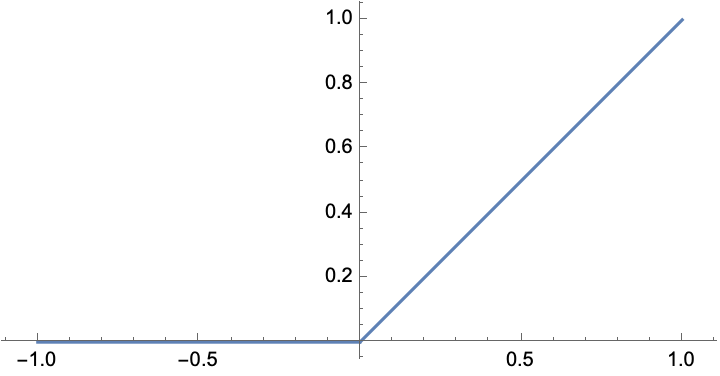
\includegraphics[width=0.7\linewidth]{1}
		\caption*{Example 1}
		\label{fig:1}
	\end{figure}
	
\end{ex}
\begin{defn}[Root]
	$r\in\R$ is a root of a polynomial $f$ if we can write \begin{align*}f(x)=``\sum_{i=0}^d=c_ix^i"=\max_{i=0}^d\{c_i+ix\}\end{align*}
	and $\max$ is reached of at least two monomials.
	That is, $r\in\R$ is a root if the function defined by $f$ is not lineal in a neighbourhood of $r$.
\end{defn}
Which corresponds to the root 0 of the polynomial in our example.
\begin{ex} Take the polynomial
	$$``0+(-1)x+x^2"$$
	\begin{figure}[H]
		\centering
		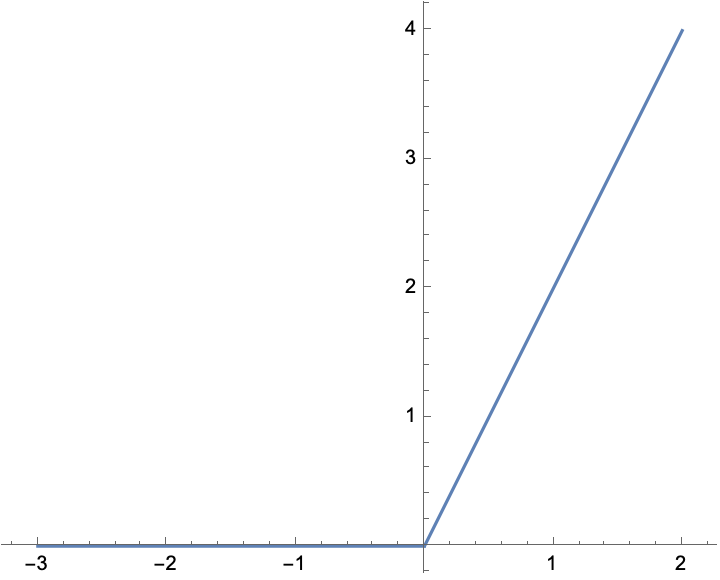
\includegraphics[width=0.5\linewidth]{2}
		\caption{}
		\label{fig:3}
	\end{figure}
	
	0 is a root of multiplicity 2, for 2 is the distance between the monomials that are not ``ghosts'' in the polynomial. Only -1 is a ghost coefficient, and the distance between 0 and 2 is 2.
\end{ex}
\begin{ex}
	Take
	$$``0x+1\cdot x+x^2"=\max\{0,x+1,2x\}$$
	Now we have two singularities, which ammount to two roots, and now both have multiplicity 1.
	\begin{figure}[H]
		\centering
		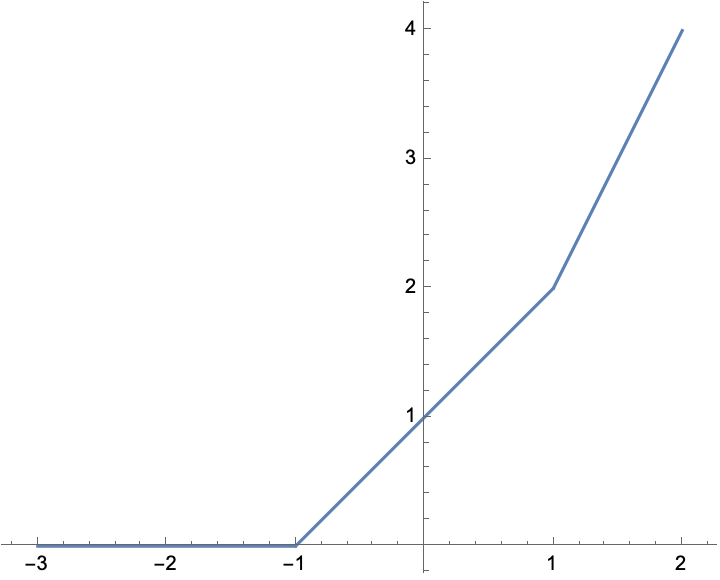
\includegraphics[width=0.5\linewidth]{3}
		\caption*{Example 3}
		\label{fig:2}
	\end{figure}
\end{ex}
\begin{defn} For $f(x)=``\sum_{i=0}^da_ix^i"$ and $x_0\in\R$, we define
	$$\In_{x_0}f(x)=``\sum_{i\text{ s.t. }f(x_0)=a_ix_0^i}a_ix^i"$$ and $$\mult_f(x_0)=\ell(\conv\{i:a_ix^i_0=f(x_0)\})$$
\end{defn}
\begin{ex}
	Take $$f(x)=``0+x+x^2+x^3"$$
	For $x_0<0$ we have $\In_{x_0}f(x)=0$ and $\mult_f(x_0)=0$. For $x_0>0$ we have $\In_{x_0}f(x)=``x^3"$ and $\mult_f(x_0)=0$. And for $x_0=0$ we have $\In_{x_0}f(x)=f(x)$ and $\mult_f(x_0)=3$.
	\begin{figure}[H]
		\centering
		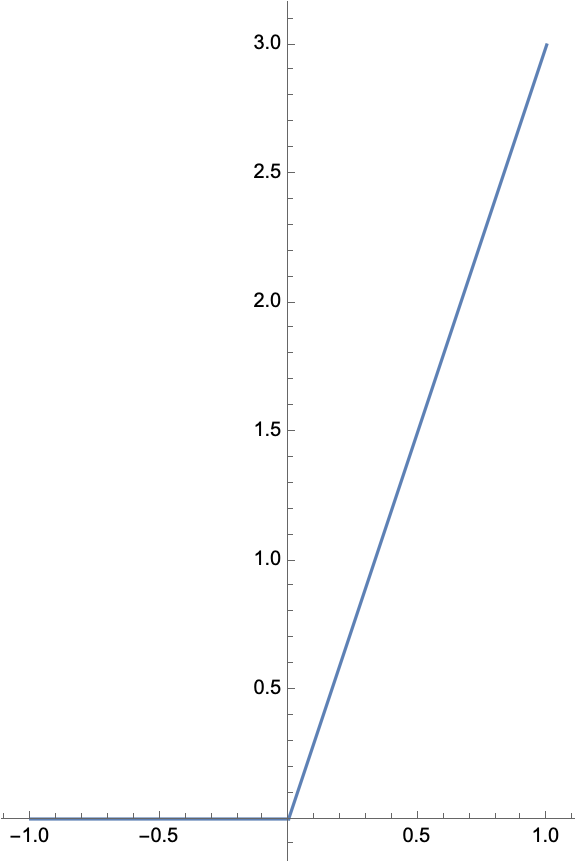
\includegraphics[width=0.3\linewidth]{6}
		\caption*{}
		\label{fig:6}
	\end{figure}
	
\end{ex}
\begin{thm*}[Fundamental Theorem of Tropical Algebra] For any polynomial of degree $d$,
	$$
	\sum_{r\text{ is a root of }f}\text{mult }r=d
	$$
\end{thm*}
Thus we now know what is the multiplicity of a root. We must agree that the multiplicity of $-\infty$ is the minimum exponent of the polynomial.
\subsection{Two variables}
\begin{ex}
	$$f(x,y)=``0+x+y"=\max\{0,x,y\}$$
	\begin{figure}[H]
		\centering
		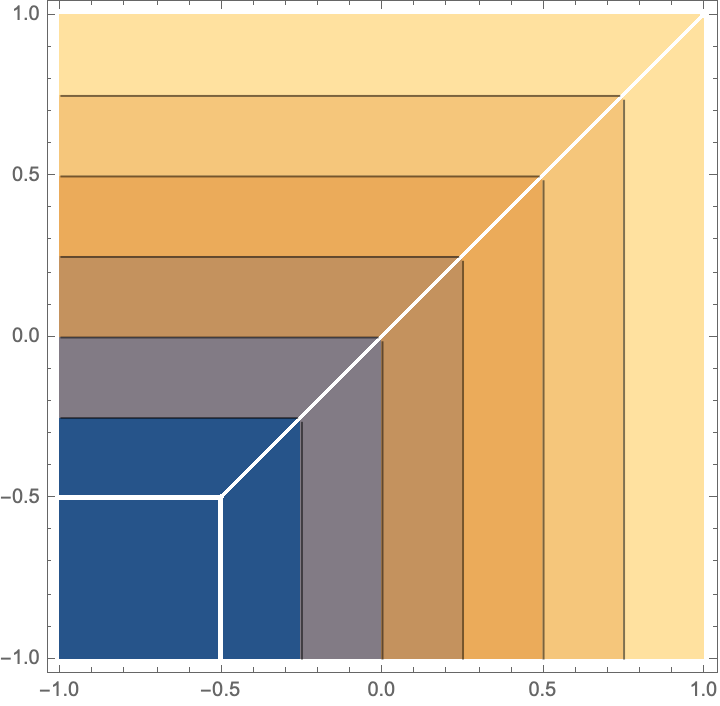
\includegraphics[width=0.4\linewidth]{7}
		\caption*{}
		\label{fig:7}
	\end{figure}
\end{ex}
\begin{defn}
	For $f(x,y)=``\sum a_{ij}x^iy^j"$ define $$\Ex_f=\{(i,j):a_{ij}\neq0\}$$
	And then the Newton Polygon is $$\conv\{\Ex_f\}$$ So its a vertex for every monomial. And finally: $$C_f:=\{(x,y):\In_{(xy)}f \text{ is not a monomial}\}$$
\end{defn}
\begin{ex}\label{ex:ex6}
	Check this one out: $$f(x)=``0+x+y+xy+x^2+y^2"=\max\{0, x + 1, y + 1, x + y + 1, 2 x, 2 y\}$$
	
	\begin{figure}[H]
		\begin{subfigure}{.5\textwidth}
			\centering
			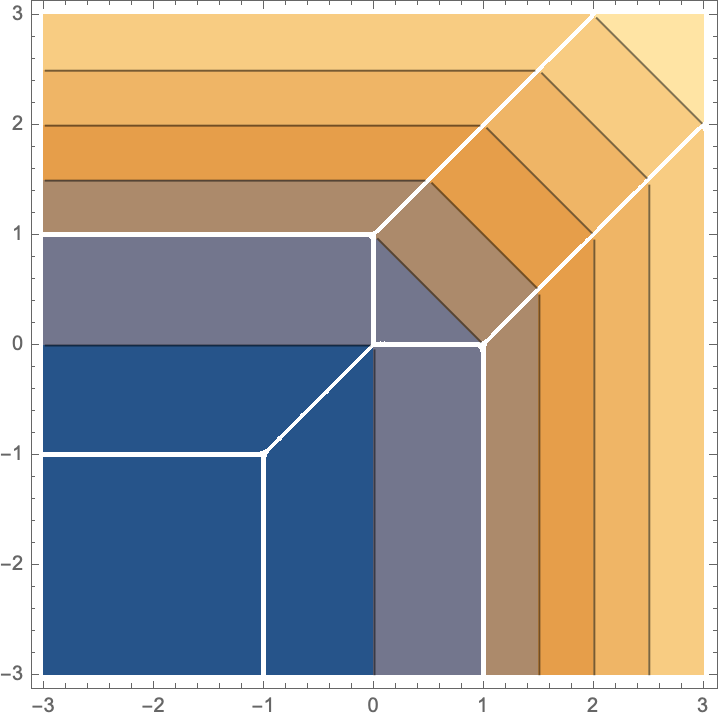
\includegraphics[width=0.9\linewidth]{8}
			\caption*{Algebraic curve}
		\end{subfigure}
		\begin{subfigure}{.5\textwidth}
			\centering
			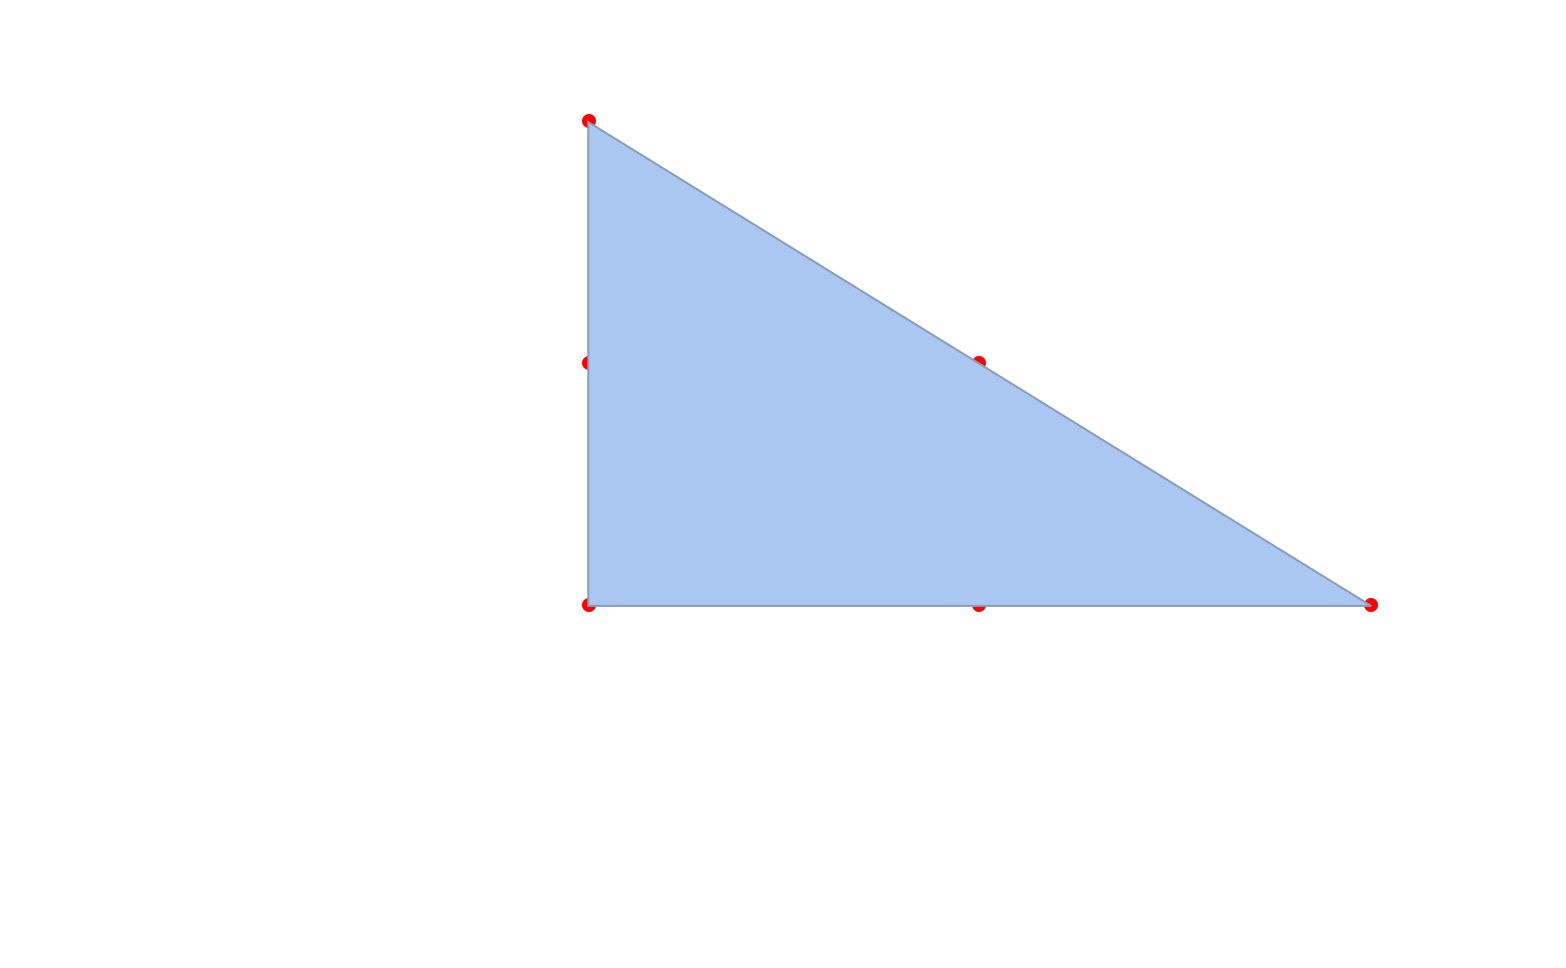
\includegraphics[width=0.9\linewidth]{9}
			\caption*{Newton polygon}
		\end{subfigure}
	\end{figure}
	Although the Newton polygon is the dual geometric object of the graph, it cannot be superposed with it because they live in different geometric spaces.
\end{ex}
Anyway let's define
\begin{defn}
	A graph in $\R^2$ is tropical if
	\begin{enumerate}
		\item Edges to rational
		\item Weights in the edges
		\item Balanced
	\end{enumerate}
\end{defn}
\begin{defn}
	Tropical hypersurface defined by $f$:
	$$
	H_f=\{p:\In_pf\text{ is not a monomial}\}
	$$
	And for an ideal $I$
	$$
	N_I=\{p:\forall f\in I, \In_pf\text{ is not a monomial}\}
	$$
\end{defn}
\subsection{Tropicalization}
We will learn how to use tropical geometry to study classical geometry. How can we go from classical polynomial to tropical ones?\par
Let's take a classical polynomial in $\C[X]$ and induce a tropical polynomial:
$$
F(X)=\sum_{i=0}^dA_iX^i\rightsquigarrow f(x)=``\sum_{i=0,A_i\neq0}^dx^i"
$$
It looks to me that you basically get rid of the coefficients and then take the tropical operations.\par 
Now let's try making the coefficients functions of $t$:
$$
F_t(X)=\sum_{i=0}^dA_i(t)X^i\rightsquigarrow f(x)=``\sum_{i=0,A_i\neq0}^d(-\gamma_1) x^i":=F^\trop
$$
where $A_i(t)=\gamma_jt^j$.\par
So this time you only take the first coefficient. \textit{Is there anything to correct here?}\par
\begin{ex}
	$$
	3t^0+4t^0x+x^2+x^3+y+t^1xy+x^2y+
	$$
\end{ex}
\begin{thm}[Kaparanov]
	$$
\begin{tikzcd}
	F_t \arrow[r, "\text{zeroes}"] \arrow[d, "\text{tropicalization}"'] & \text{Surface of genus }g\arrow[d, "\text{amoeba: }\Log_t\text{ then }t\to0"] \\
	f \arrow[r, "\text{zeroes}"'] &\begin{tabular}{c}  \text{Tropical curve with }\\ $g$\text{ bounded regions} \end{tabular}
\end{tikzcd} $$
And then we can calculate the Newton Polygon and do combinatorics.
\end{thm}

\subsection{Enumerative Geometry}
$$
N_\C(\delta,p)=N_\T(\delta,p)
$$
\subsection{Matroids}
\begin{defn}[Matroid]
	$E\neq\emptyset$, $B$ a set of bases that satisfies the Exchange property, that is, for $B_1,B_2\in B$, there always exists $e_1\in B_1$ and $e_2\in B_2$ such that $B_1\backslash e_1\cup e_2\in B$.
\end{defn}
\iffalse
Let us include Wikipedia's definition for further clarity:
\begin{defn}
	A (finite) matroid is a pair $(E,\mathcal I)$ with $E$ a nonempty finite set and $\mathcal I$ a family of subsets of $E$ called the \textbf{independent sets} with the following properties:
	\begin{enumerate}
		\item The empty set is independent, that is, $\emptyset\in \mathcal I$.
		\item Every subset of an independent set is independent, that is, for $A'\subseteq A\subseteq E$, si $A\in\mathcal I$, then $A'\in\mathcal I$. This is the \textbf{hereditary property}.
		\item If $A$ and $B$ are independent sets and $A$ has more elements than $B$, then there exists $x\in A\backslash B$ such that $B\cup \{x\}$ is in $\mathcal I$. This is the \textbf{indendependent set property}.
	\end{enumerate}
\end{defn}
\fi
\begin{ex}
	Let  $E=\{a,b,c,d,e\}$ and $B=\{\{a,b,c\}.\{a,b,d\}.\{a,b,e\},\{a,c,d\},\{a,c,e\}\}$. For every base lets produce a vector that has 1 if the base contains the element in the corresponding slot according to the order $(a,b,c,d,e)$. So for example the first base has vector $(1,1,1,0,0)$.\par
	This produces five vectors in $\R^5$ whose convex hull is a polyhedron.
	\begin{figure}
		\centering
		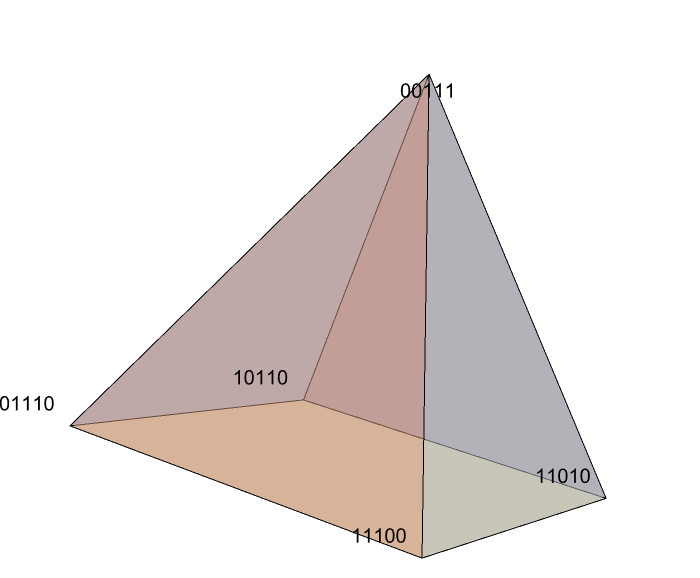
\includegraphics[width=0.5\linewidth]{10}
		\caption*{}
		\label{fig:10}
	\end{figure}
	Now it turns out that the independent set property lets us direct the edges in this polytope. 
	%\paragraph{I think that }for example take the bases $11100$ and $11010$ choosing the first entry in both bases and applying our property in the definition of matroid we end up with the base $01110$ so we have an arrow from $11100$ to $01110$.
\end{ex}
\begin{defn}
	$\Delta$ is a matroidal polytope if all the edges of $\Delta$ are in direction $e_j-e_i$ for some $i,j$.
\end{defn}
Actually there is a bijection between matroids and these directed polytopes.
\begin{ex}[Bergman fan, Ardila, Klivans]
	$E$ of size 5, and a family in $\R^4$. Let us associate:
	\begin{align*}
		a\rightsquigarrow(-1,0,0,0)\qquad b\rightsquigarrow(0,-1,0,0)\qquad c\rightsquigarrow(0,0,-1,0)\qquad d\rightsquigarrow(0,0,0,-1) \qquad e\rightsquigarrow(1,1,1,1)
	\end{align*}
\end{ex}

\begin{ex}[Balanced (Tropical) fan]
	$E$ of size 3, say $E=\{0,1,2\}$ and $B=\{\{0\},\{1\},\{2\}\}$. Let us associate:
	\begin{align*}
		0\rightsquigarrow(1,1)\qquad 1\rightsquigarrow(-1,0)\qquad 2\rightsquigarrow(0,-1)
	\end{align*}
	And this produces
	\begin{figure}[H]
		\centering
		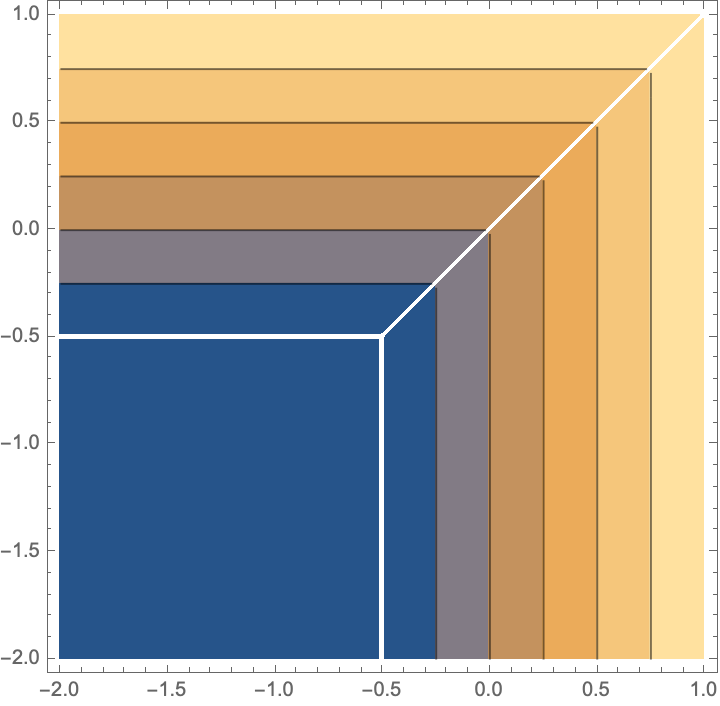
\includegraphics[width=0.4\linewidth]{11}
		\caption*{}
	\end{figure}
	Where every line is a ray spanned by the three vectores we chose. This is the Tropical Fan.
\end{ex}
And it turns out matroids are the same as tropical fans of degree 1. And also there's the polytope idea so we have these three definitions.
Another example of a tropical fan is the tropical curve in Example \ref{ex:ex6}.
\newpage
\subsection{Three examples (extra)}
\begin{ex}
	Here are the roots of the classical polynomial $x^2+y^2-1$ (with the usual operations in $\R[x,y]$) and its plot in $\R^3$:
	\begin{figure}[H]
		\begin{subfigure}{.5\textwidth}
			\centering
			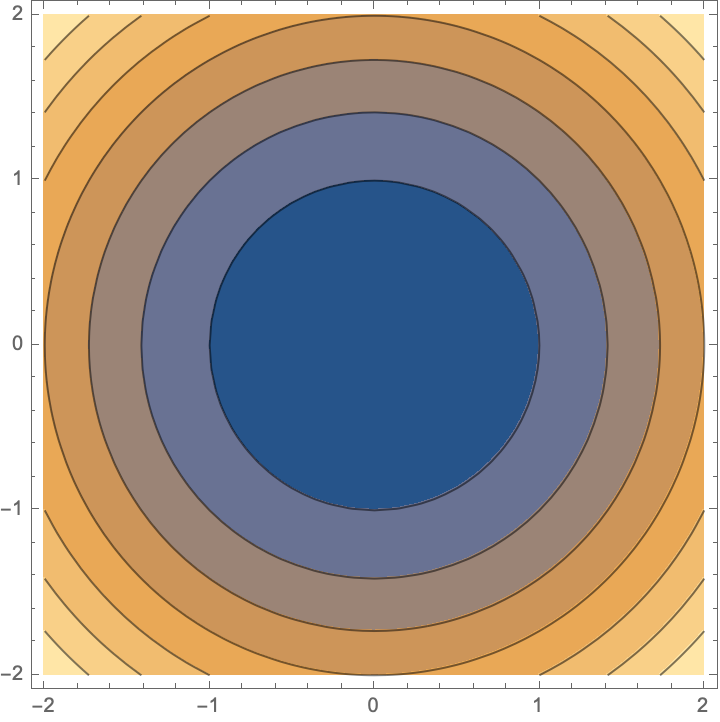
\includegraphics[width=0.9\linewidth]{dani1}
		\end{subfigure}
		\begin{subfigure}{.5\textwidth}
			\centering
			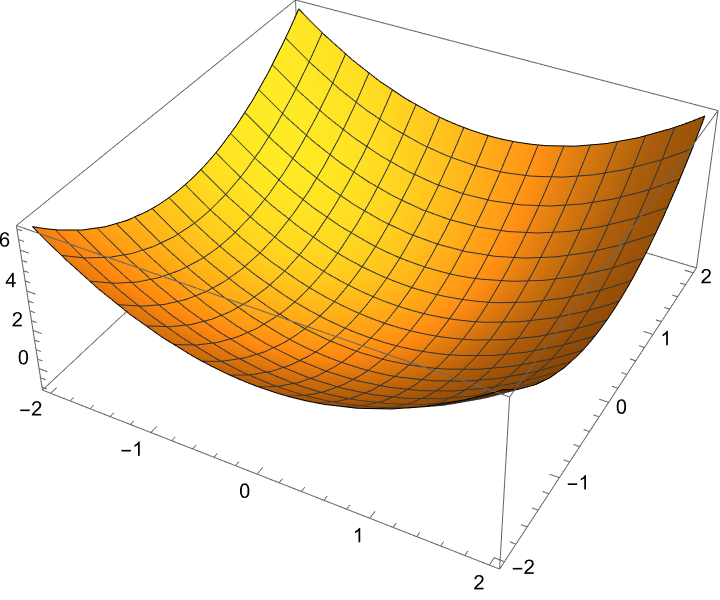
\includegraphics[width=0.9\linewidth]{dani2}
		\end{subfigure}
	\end{figure}
	And now we do exactly the same but for the tropical polynomial $``x^2+y^2-1"=\max\{2x,2y,0\}$:
	\begin{figure}[H]
		\begin{subfigure}{.5\textwidth}
			\centering
			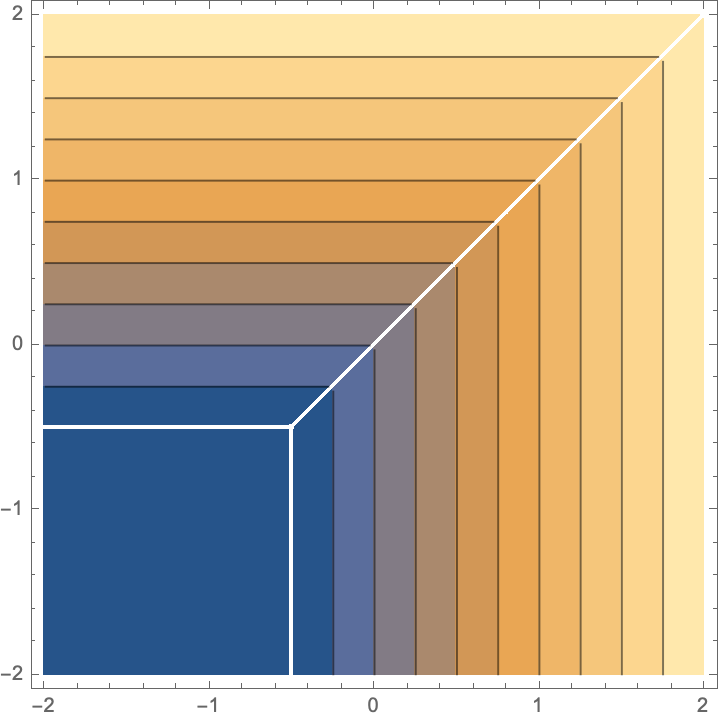
\includegraphics[width=0.9\linewidth]{dani3}
		\end{subfigure}
		\begin{subfigure}{.5\textwidth}
			\centering
			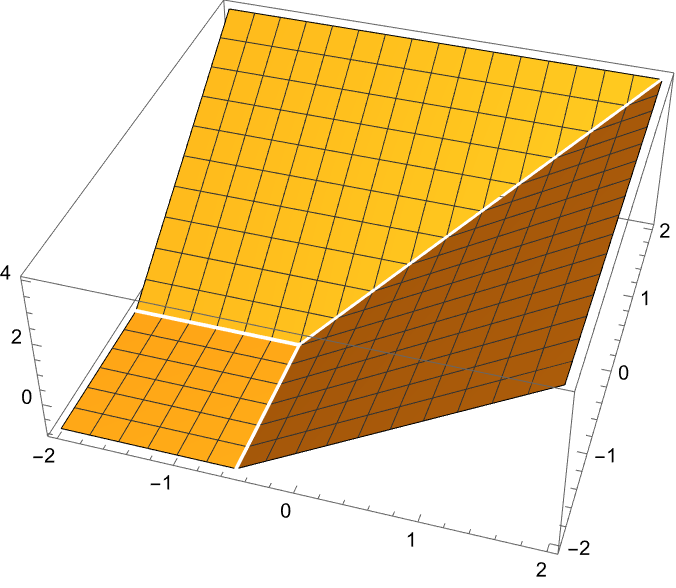
\includegraphics[width=0.9\linewidth]{dani4}
		\end{subfigure}
	\end{figure}
\end{ex}
\begin{ex}
	Here are the roots of $x^3 + 2 xy + y^4\in\R[x,y]$ and a related tropical polynomial $``x^3 + 2 xy + y^4+0"=\max\{3 x, 2 + x + y, 4 y,0\}$:
	\begin{figure}[H]
		\begin{subfigure}{.5\textwidth}
			\centering
			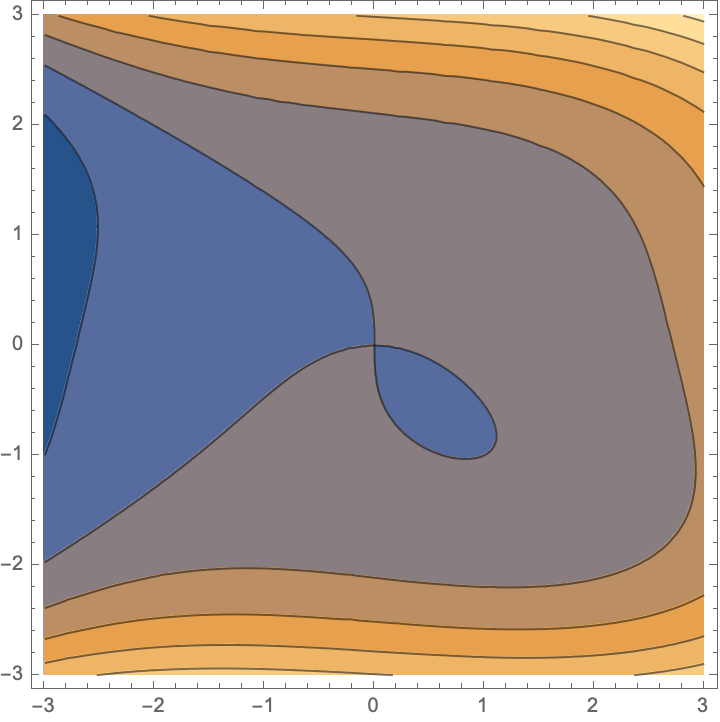
\includegraphics[width=0.9\linewidth]{dani5}
		\end{subfigure}
		\begin{subfigure}{.5\textwidth}
			\centering
			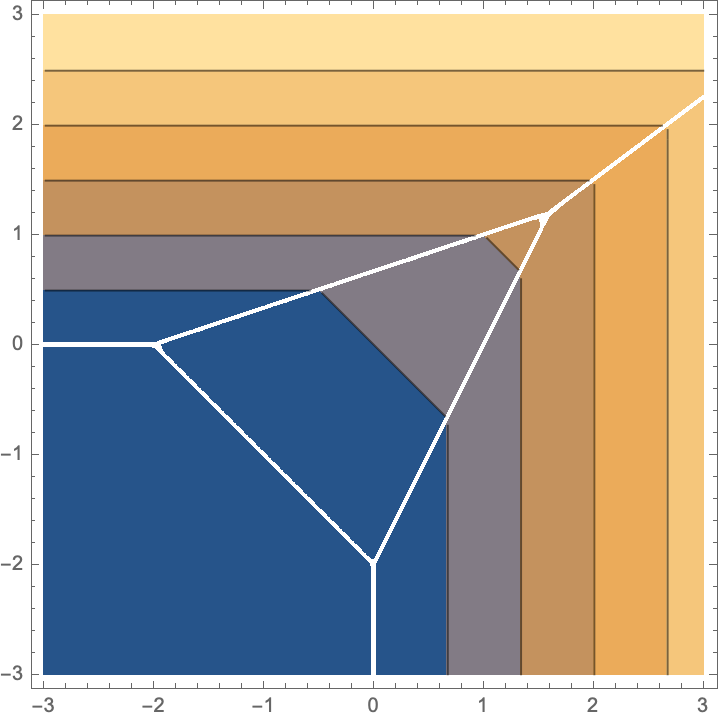
\includegraphics[width=0.9\linewidth]{dani6}
		\end{subfigure}
	\end{figure}
	Notice we must include the 0 in the tropical polynomial, because without it we do not get the triangle in the plot.
\end{ex}

\newpage
\subsection{Benoit's talk on Real tropical geometry}
Let us define a family of polynomials of degree $d$ parametrized by $t$:
$$
p_t(x,y)=\sum_{i+j\leq d}c_{i,j}t^{v_{i,j}}x^iy^j
$$
Now consider de map
\begin{align*}
	\Log_t:(\C^\times)^2&\to\R^2\\
	(x,y)&\mapsto \Big(\frac{\log |x|}{\log t},\frac{\log|y|}{\log t}\Big)
\end{align*}
And then define for a curve $\mathcal C\subset(\C^\times)^2$ the amoeba of $\mathcal C$ as $\Log_t(\mathcal C)$. Notice $\mathcal C$ is a \textit{complex} curve, which is a real surface. So the image of our function is a region in $\R^2$.\par
Here's Dani's incomplete attempt of an amoeba:
\begin{figure}[H]
	\centering
	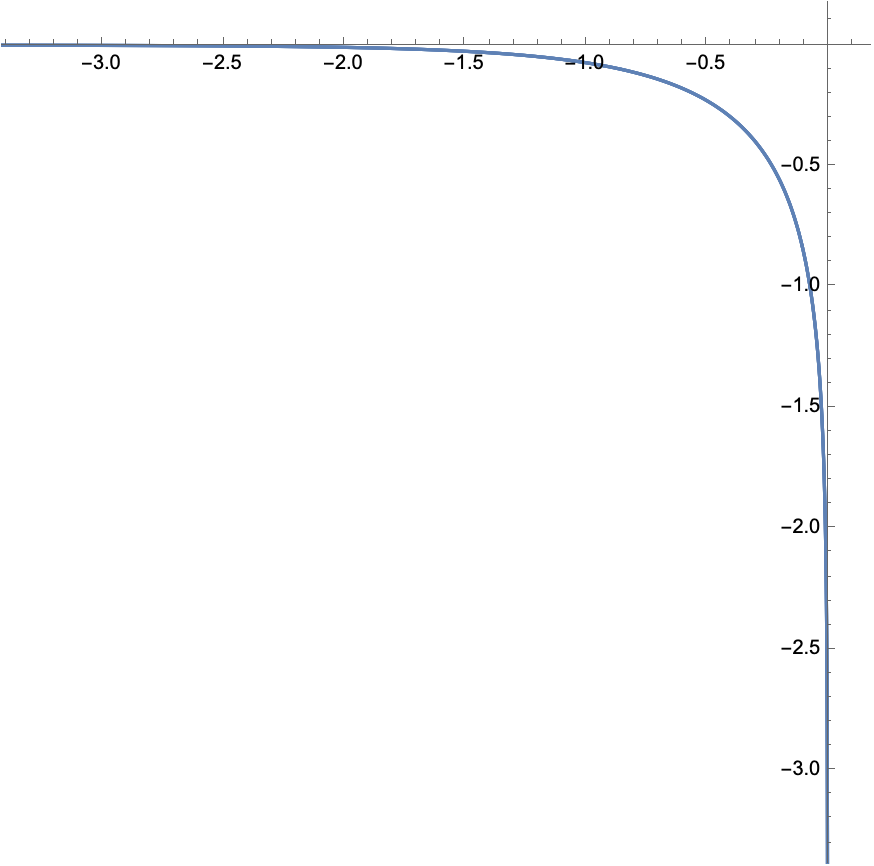
\includegraphics[width=0.5\linewidth]{amoeba1}
	\caption*{}
	\label{fig:amoeba1}
\end{figure}
And now define as in Lucía's talk:
$$
\mathfrak p=``\sum_{i+j\leq d}c_{ij}x^iy^j"=\max_{i+j\leq d}\{c_{ij}+ix+jy\}
$$
Taking edges as perpendicular lines to edges in a tropical conic, and vertices as the centres of regiones determined by the conic, we obtain a subdivision of the plane that looks like the dual tiling of the conic.\par 
\begin{obs} The genus of the curve equals the ammount of bounded regions determined by the tropical curve.
\end{obs}
Then he takes the amoebas of the real parts of curves and he obtains plane curves. He then 'unfolds' these curves by taking each part of the curve that is lying in each of the four quadrants of the plane, and then he pastes back each of these pieces.\par
And then take the limit as $t\to\infty$ and finally folding them back. This is some sort of combinatorial procedure. And it turns out that:
\begin{thm*}[Viro, 1976]
	$$(\R^2,T_\R)\cong(\R^2,\mathcal C_\R)$$
	where $\cong$ is homeomorphic. So they have the same Newton polygon and same degree.
\end{thm*}
Where $T_\R$ is the real part he's been working with in the last two paragraphs and $\mathcal C_\R$ looks like the whole complex curve (real surface).
\begin{ex}[Dani's attempt to use Benoit's Log function]
	Let us try to evaluate our $\Log_t$ function in a complex algebraic curve. We must remember that the zeroes of polynomials of the form $y^2=\prod_{k=1}^{2g+1}(x-a_k)$ are called \textit{hyperelliptic curves} when $g>1$ and \textit{elliptic curves} when $g=1$ (According to \cite{diez}).\par
	Taking $g=1$, we have a curve of genus 1, that is, a torus. We hope that when we evaluate $\Log$ in this torus we get exactly one bounded region in the resulting drawing. The polynomial in this case is 
	$$y^2=(x-a_1)(x-a_2) (x-a_3)
	$$\hfill(Unfinished)\par
\end{ex}
\subsection{An exercise on tropical geometry}
 We are interested in the following figure:
 \begin{figure}[H]
		\centering
		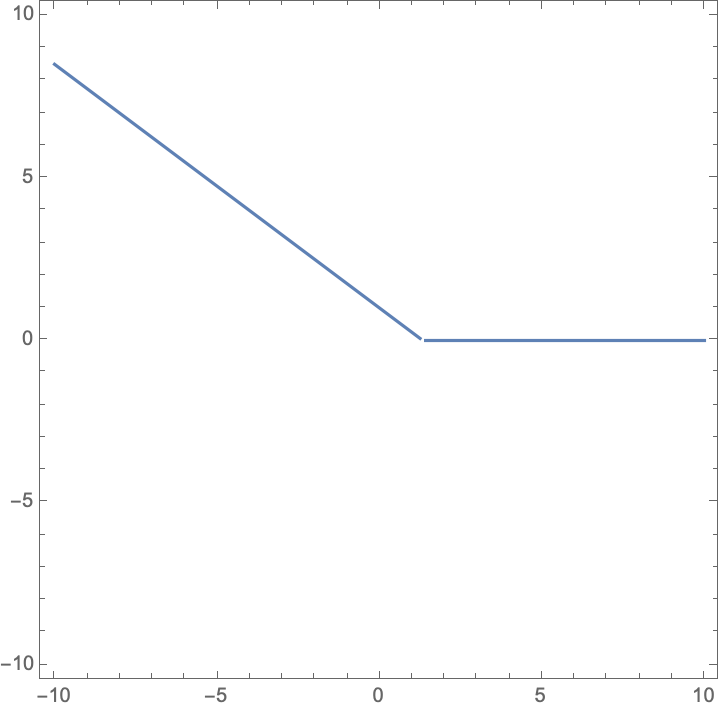
\includegraphics[width=0.4\linewidth]{Notas2/Exercise on tropical geometry/ex1.png}
		\label{ex1}
	\end{figure}
 It represents the nullcline of some system of differential equations (See \cite{curto2},\cite{curto1}).\par
 Also it is the zeroes of the classical (non-tropical) function
	$$
	-y+\max\{1-\frac{3}{4},0\}=0
	$$
	How can we make it into a tropical curve?
	

	Benoit shows how it is contained in the zeroes of the tropical polynomial $``0-4x^3-4x^3y^4"$, using its Newton Polygon:
	
	\begin{figure}[H]
		
		\begin{subfigure}{0.5\textwidth}
				\centering
				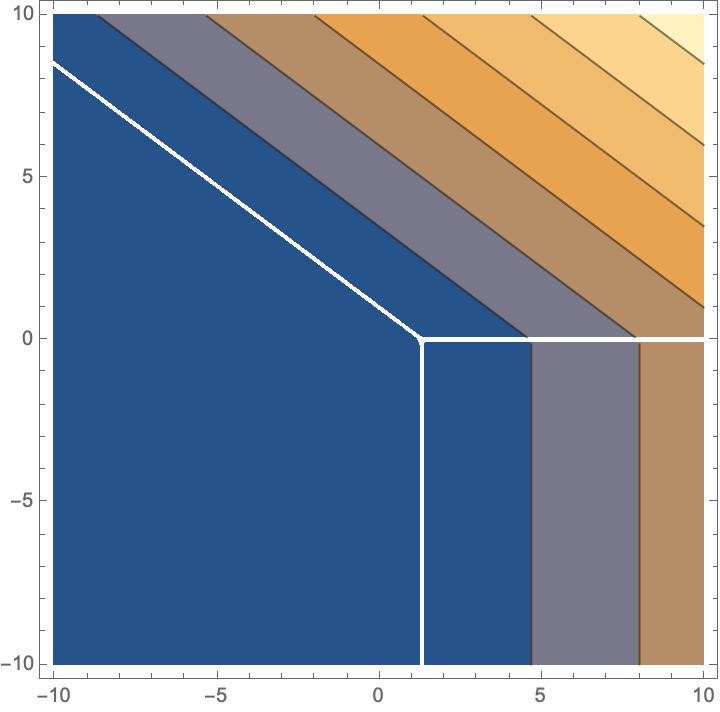
\includegraphics[width=0.8\linewidth]{Notas2/Exercise on tropical geometry/ex2.png}
				\label{ex2}
		\end{subfigure}
		\begin{subfigure}{0.5\textwidth}
			\centering
			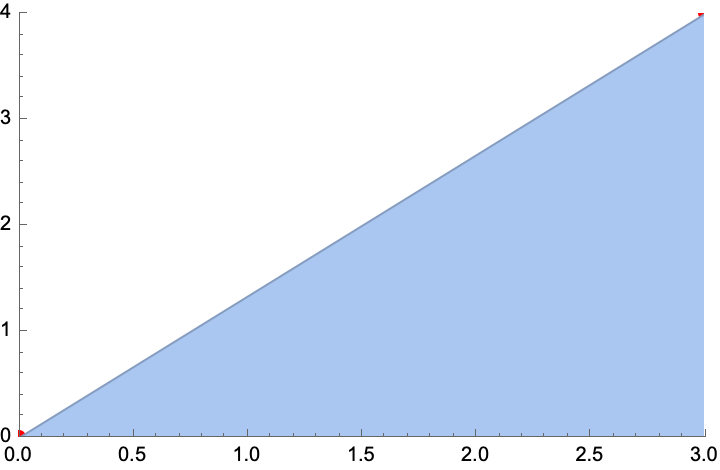
\includegraphics[width=0.8\linewidth]{Notas2/Exercise on tropical geometry/ex3.png}
			\label{ex3}
		\end{subfigure}
	\end{figure}

 Here's how he did it:

 \begin{figure}[H]
		\centering
        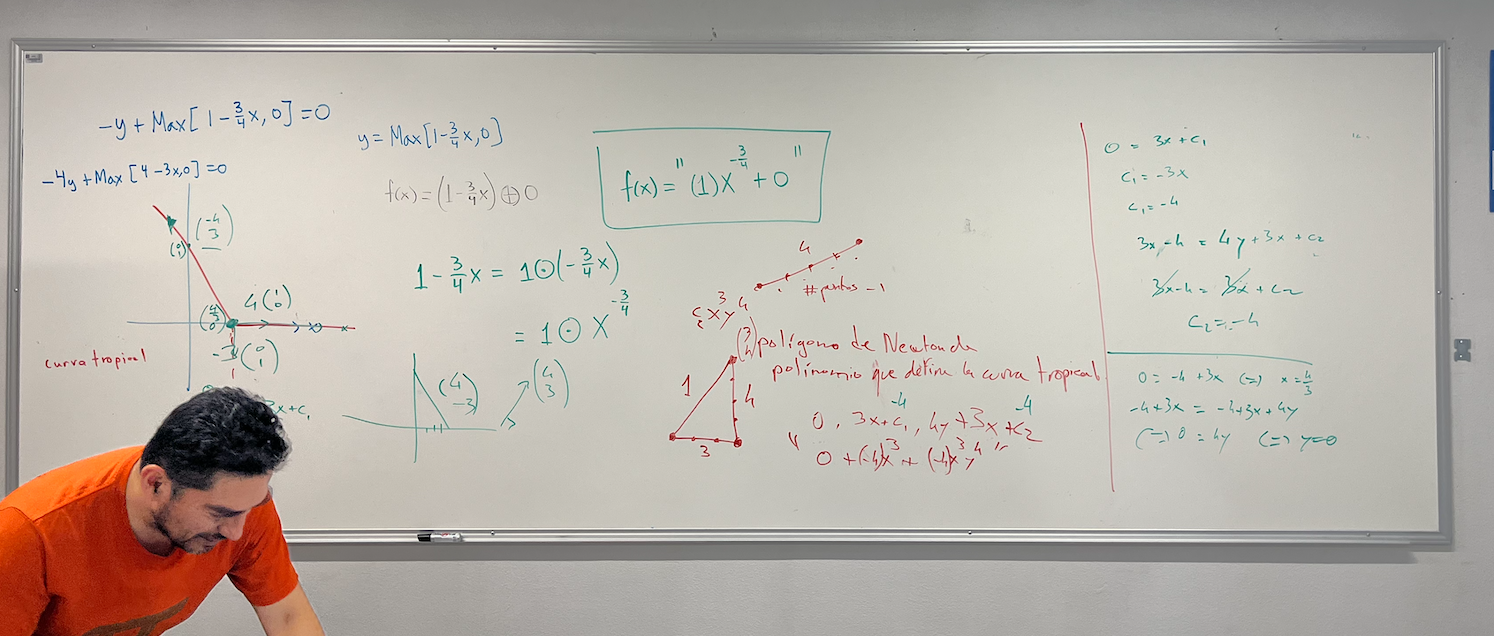
\includegraphics[width=1\linewidth]{Notas2/Exercise on tropical geometry/ex4.png}
		\label{fig:ex4}
	\end{figure}

 We next wonder, in the context of our nullcline original problem, what happens when we reflect the curve in the \hyperref[ex1]{first figure} with respect to the identity line? Is there a way to repeat the process? Can we reflect the \hyperref[ex2]{second figure} by the identity line and find the tropical polynomial whose zeroes is this curve?\par
 Here's Benoit's unfinished attempt:

\begin{figure}[H]
		\centering
        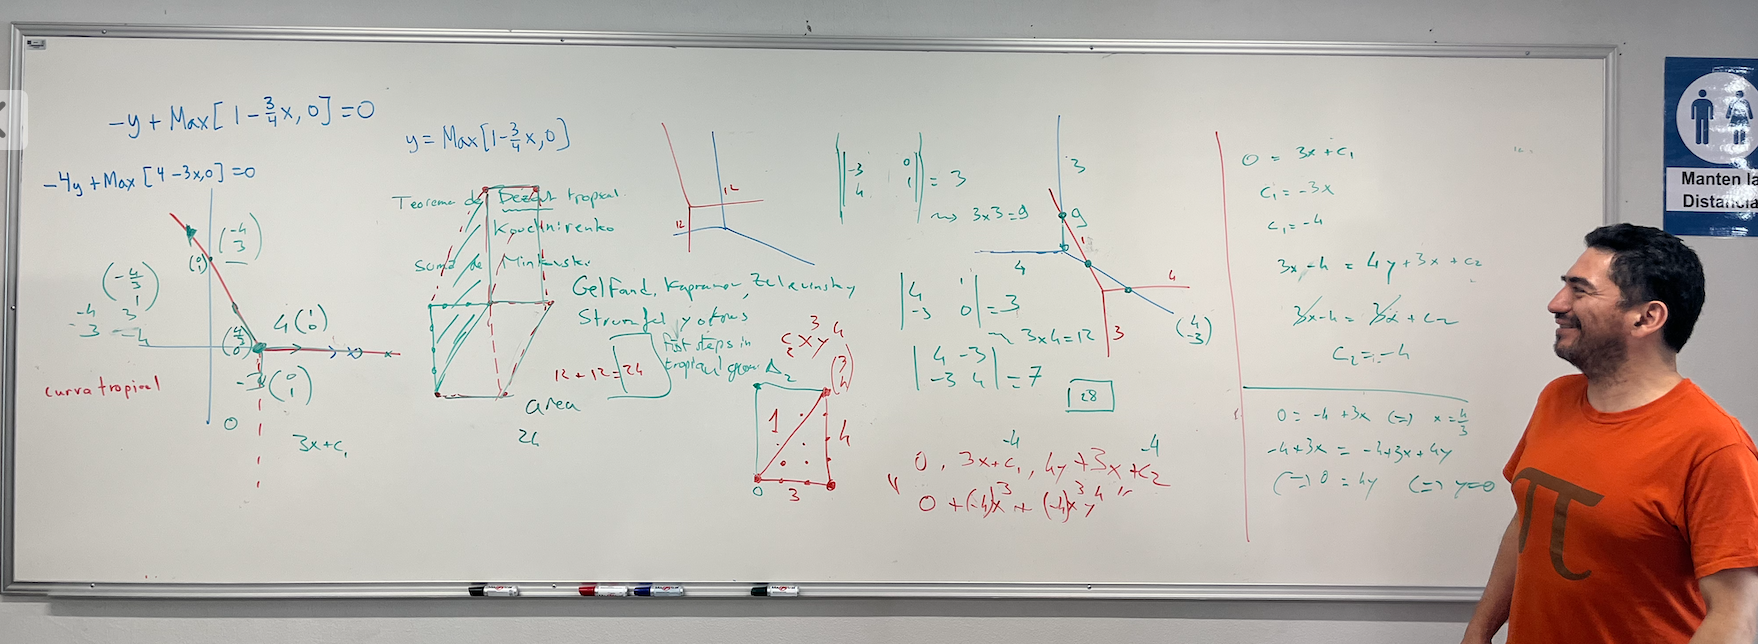
\includegraphics[width=1\linewidth]{Notas2/Exercise on tropical geometry/ex5.png}
		\label{ex5}
	\end{figure}
 
	Check Bezout Kouchurneko, Tropical. Also Gelfand Kapranov Zelvinsky and Strunfel y otros, First setps in tropical geometry.	
\subsection{Open problems}
\begin{enumerate}
    \item Not every tropical object can be obtained using the $\Log_t$ and $t\to\infty$ method (limits of amoebas). Which tropical objects can?
    \item Find correspondence theorems between classical and tropical geometry like Mikhalkin's (\cite{mikhalkin2006tropical}?)
    \begin{itemize}
        \item  Number of curves passing through a number of points.
        \item Try finding a reference ``Welschinger GW, Gromov Witten"
    \end{itemize}
    \item When can Viro Pachworking work? That is, find real algebraic objects with the same topology as algebraic varieties.
\end{enumerate}
And what's up with genus 2 cubics?
\newpage

\newpage
\section{Computational commutative algebra}
Matías Bender, matiasbender@inria.fr
\subsection{Univariate polynomials and resultants}
$R$ a ring, like polynomials. It should be commutative and an integral domain ($a,b\in\R\backslash\{0\}\implies ab\neq0$). Also take a field $\K$ and its algebraic closure $\bar\K$.
\subsubsection{Univariate polynomials}
Take the polynomial ring $k[x]$ and $f\in k[x]$ with $f=\sum_{i=0}^dc_ix^i$ for $c_i\in k$ and $c_d\neq 0$. We say $\deg f=d$.\par
Now let $k\subseteq \K$ and $p\in\K$ we define $f(p)=\sum_i c_i p^i\in\K$ the evaluation of $f$. And we say a root of $f$ is $p$ such that $f(p)=0$.\par
\paragraph{Question} Given $f_1,...,f_r\in k[x]$, do they have a common root?
\begin{defn}
	Given $f_1,...,f_r\in k[x]$ we define the ideal $\langle f_1,...,f_r\rangle=\{\sum g_if_i:(g_1,...,g_r)|in k[x]\}$
\end{defn}
\begin{prop}
	Let $p\in \K$. $\forall f\in\langle f_1,...,f_r\rangle$, $f(p)=0\iff f_i(p)=0\forall i$.
\end{prop}
\begin{obs}
	If $g\in\langle f\rangle$, then if $p\in\K$ is such that $f(p)=0$ then $g(p)=0$.
\end{obs}
\begin{prop}
	Given $f,g\in k[x]$, there are unique $(q,r)\in 
	k[x]^2$ such that $f=q\cdot g+r$ and $r=0$ or $\deg r <\deg g$.\par
	We define $\text{rem } (f,g)=r$ and write $f|g$ if and only if $\text{rem }(f,g)=0$.
\end{prop}
\begin{thm}
	$k[x]$ is a principal ideal domain. That is, for every ideal $\langle f_1,...,f_r\rangle$ there exists one polynomial $g$ such that $\langle f_1,...,f_r\rangle=\langle g \rangle$. $g$ is called GCD of $f_1,...,f_r$.
\end{thm}
I challenge to prove that
\begin{prop}
	$GCD(f_1,...,f_r)$ is the smallest polynomial with degree such that if $(\forall i)h|f_i$, then $h|GCD(f_1,...f_r)$.
\end{prop}

\begin{algorithm}[H]
\caption{Euclidean Algorithm}
	\SetKwInOut{Input}{Input}
	\SetKwInOut{Output}{Output}
	
	\Input{$f, g\in k[x]$ with $\deg f\geq\deg g$}
	\Output{$r\in k[x]$ such that $\langle f,g\rangle=\langle r\rangle$}

 		\If{$r_{-1}=f,r_0=g,i=0$}{
			$i=i+1\qquad
			r_i=\text{rem}(r_{i-2},r_{i-1})$}\;
	\Return{$r_{i-1}$}\;
\end{algorithm}

\begin{thm}
	Euclidean Algorithm terminates and is correct.
\end{thm}
\begin{proof}
	It terminates because $\forall i\geq1)$ $\deg(r_i)>\deg(r_{i+1})$ Hence $\exists i_*$ such that $r_{i_*}=0$. Observe that for each $i$, $\exists q_i\in k[x]$ such that $r_{i-2}=r_{i-1}q_i+r_i$. Hence $\langle r_{i-2},r_{i-1}\rangle=\langle r_{i-1},r_i\rangle$.\\
	$h_1r_{i-2}+h_2r_{i1}\iff(h_1q_1+h_2)r_{i-1}+h_ir_i$.\\
	Therefore, $\langle f,g\rangle=\langle r_{-1},r_0=....)\langle r_{k-1},r_{i_*}\rangle$
\end{proof}
\paragraph{HW}
	Prove that $GCD(f_1,f_2,f_3)=GCD(GCD(f_1,f_2),f_3)$.
\paragraph{Conclusion} If $GDC(f_1,...,f_r)=1$, then there are no common solutions.\\
If $GCD(f_1,...,f_r)\neq 1$. Then $f_1,...,f_r$ have ea common factor if $k=\bar k$ and $\exists p\in k$ such that $f_1(p)=...=f_r(p)=0$.\par

Now consider a UFD ring $R$ like $\C[y],\C[x,y]$.
\begin{defn}[Resultant]
	Given $f(x,y)=\sum_{i=1}^m f_i(y)x^i \in\C[x,y]$ that is, $f\in\C[y]$, and $g=\sum_{i=1}^m g_i(y)x^i$. We define Sylvester matrix $\text{Sylv }(f,g,x)$.\\
	\begin{align*}
		\begin{pmatrix}f_m&0&...&0&g_m&0&...&0\\ 
			f_{m-1}&f_{m}&...&0&g_{m-1}&g_{m}&...&0\\
      &&...&&&&...&\\
			f_0 & f_1&...&f_m&g_0 & g_1&...&g_m\\
			0&f_0&...&f_{m-1}&0&g_0&...&g_{m-1}\\
         &&...&&&&...&\\
   			0&0&...&f_0&0&0&...&g_0\\
		\end{pmatrix}
	\end{align*}\par
	The resultant $Res(f,g,x)=\det \text{Sylv }(f,g,x)\in \C$.
\end{defn}
We may substitute $\C$ with any ring $R$.
\begin{obs}
	$\text{Sylv }(f,g,x)$ represents $\bar{\text{Sylv }_{f,g,x}}(A,B)\mapsto Af+Bg=\sum c_ix^i$ with $c_i\in\R$. Where $\deg_x(A)<\deg_x(g)$ and $\deg_x(B)<\deg_x(f)$. So $A$ and $B$ are polunomials of the form $A=\sum_{i=0}^{m-1}A_ix^i$ and $B=\sum_{i=1}^{m-1}B_ix^i$.  So with two polynomials I obtain another polynomial.
\end{obs}
\begin{prop}
	$\Res{f,g,x}=\img \Sylv _{f,g,x}$ that is, $\exists A,B$ such that $\deg A<\deg g$, $\deg B<\deg A$ such that $Af+By=\Res (f,g,x)$.
\end{prop}
\paragraph{HW} Prove it. Use adjugate matrix of $\Sylv(f,g,x)$.
\begin{prop}
	If $f,g\in k[x]$. The $\Res (f,g,x)=0\iff GCD(f,g)\neq1$.
\end{prop}
\subsubsection{Solving bivariate polynomial systems}
\begin{ex}
	
	$$\Sylv(f,g)=\begin{pmatrix}
		y&0&2y&0\\
		y^2+y&y&0&2y\\
		1&y^2+y&-y^2+3&0\\
		0&1&0&y^2+3
	\end{pmatrix}$$\\
	Then $\Res (f,g,x)=\underbrace{y^2}_{\text{does not lead to a solution}}\underbrace{(2y^2-3y-1)(y+1)^3}_\text{lead to solutions!}$
\end{ex}
\begin{thm}
	If $(p_x,p_y)\in\C^2$ are such that $f(p_x,p_y)=g(p_n,p_y)=0$ then $\Res (f,g,x)|_{y=p_y}=0$.
\end{thm}
\begin{proof}
	$\exists A,B$ such that $Af+Bg=\Res(f,g,x)=0=\Res(f,g,x)|_{y=p_y}$.
\end{proof}
\begin{thm}[Extension theorem] Given $f,g\in\C[x,y]$ as before, let $p_y$ be such that $\Res (f,g,x)|_{y=p_y}=0$. Then if $f_m(p_i)\neq 0$ or $g_m(p_y)\neq 0$, then $\exists p_x$ such that $(p_x,p_y)$ is solution of $f(x,y)=g(x,y)=0$.
\end{thm}
\subsection{Ideals and varieties}
\begin{ex}
	Consider the polynomials
	\begin{align*}
		f_1=x^2+4y^2-4\\
		f_2=x^2+y^2-4\\
		f_3=x^2-y-4
	\end{align*}
	How can we verify that $f_3$ vanishes at common zeros of $(f_1,f_2)$?
	\begin{figure}[H]
		\centering
		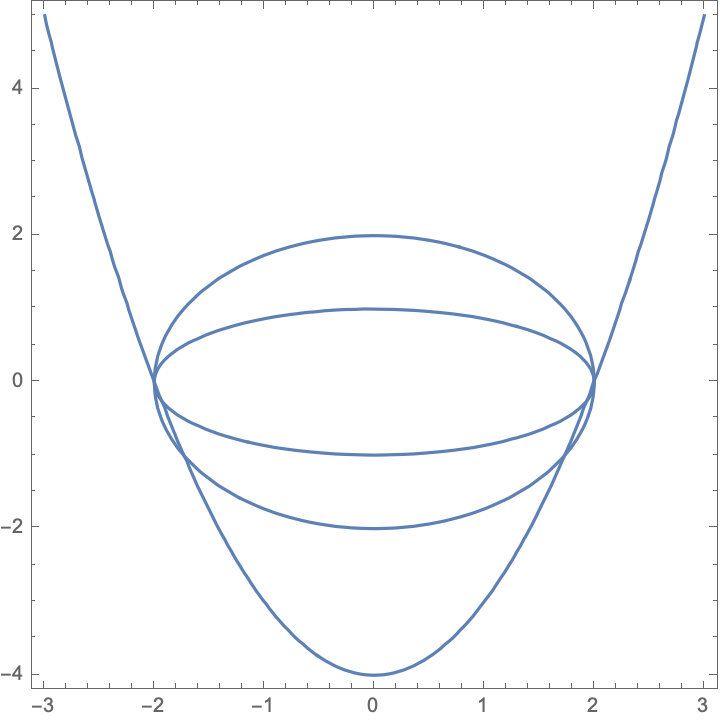
\includegraphics[width=0.5\linewidth]{4}
		\caption*{}
		\label{fig:4}
	\end{figure}
	
\end{ex}
Let $R=\C[x_1,...,x_m]$, $f \in \R$ with $f=\sum_{\alpha\in\Z_{\geq0}}c_\alpha x^\alpha$ where $c_\alpha\in\C$ there finite $\alpha$ such that $c_\alpha\neq 0$, $x^\alpha$ is monomial , $x^\alpha=\prod_{i=1}^m x_i^{\alpha_i}.$\par 
The degree is $\deg f=\max_{\alpha\in\Z_{\geq0}}(\sum\alpha_i:c_\alpha\neq0)$.\par 
	
Ok now fiven $p\in\C^m$, we can evaluate $f$ doing $f(p)=\sum c_\alpha p^\alpha.$ And we say $p$ is a zero if $f(p)=0$.\par 
\begin{defn}
	Given $f_1,...,f_r\in\R$ we define the affine algebraic variety $V(f_1,...,f_r)=\{p\in\C^m:(\forall i)f_i(p)=0\}$. And in general, if $I\subseteq R$ is an ideal, we define $$V(I)=\{p\in\C^m:(\forall i)f\in I=0\}$$.
\end{defn}

\begin{ex}
	Take
	\begin{align*}
		f_{1}&=x^2+2y^2-4\\
		f_{2}&=2xy-1
	\end{align*}
	\begin{figure}[H]
		\centering
		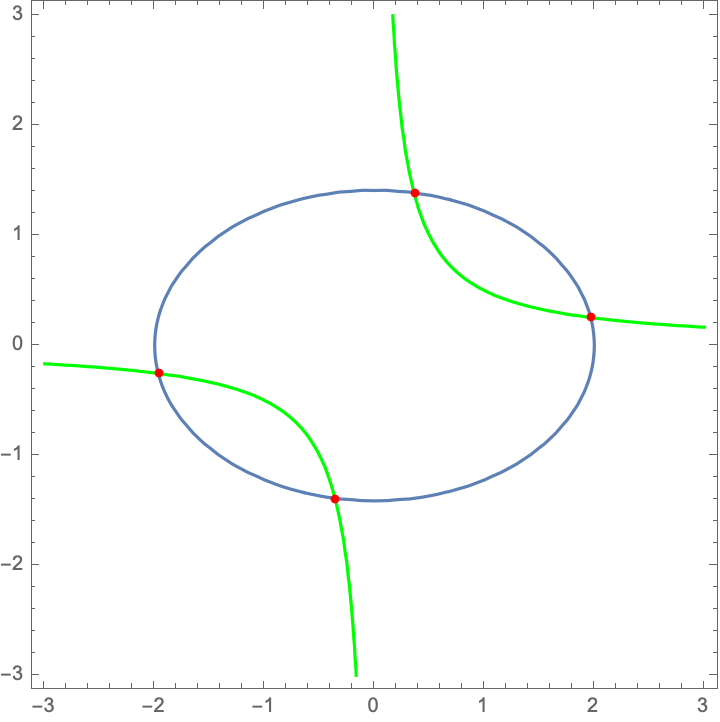
\includegraphics[width=0.5\linewidth]{5}
		\caption*{}
		\label{fig:5}
	\end{figure}
	
\end{ex}
\begin{defn}
	An ideal $I$ is a subset of $R$ such that $(\forall f,g\in I) f+g\in I$ and $(\forall f\in I)(\forall r\in \R)fr\in I$.
\end{defn}
\begin{prop}
	Given $f_1,...,f_r\in R$, we define the generated ideal as $$\langle f_1,..,f_r\rangle=\{\sum_{i=1}^rg_if_i:g_1,...,g_r\in R\}$$
\end{prop}
\begin{prop}
	$V(\langle f_1,...,f_r\rangle)=V(f_1,...,f_r)$.
\end{prop}
\begin{defn}
	The ring $R$ is Noetherian if when $I\subseteq R$ is an ideal then $\exists f_1,...,f_r$ such that $I=\langle f_1,...,f_r\rangle$.
\end{defn}
\subsubsection{Operations on ideals}
\begin{prop}Fix $I,J\subseteq R$ ideals. Then:
\begin{enumerate}
	\item $I\subseteq J\implies V(J)\subseteq V(I)$
	\item $I+J=\{f+g:f\in I,g\in J\}$ is an ideal.
	\item $I\cap J$ is an ideal and $V(I\cap J)=V(I)\cup V(J)$.
\end{enumerate}
\end{prop}
\subsubsection{Hilbert's Nullstellensatz}
\begin{defn}
	Let $W\subseteq\C^n$, we define the ideal $$I(W)=\{f\in R:(\forall p\in W)f(p)=0\}$$.
\end{defn}
\begin{prop}
	Given $W\subseteq \C^n$, $V(W)$ is the smallest with inclusions of the affine algebraic varieties that contain $W$. If $W\subseteq Z$ and $Z$ variety, then $V(I(W))\subseteq Z$. Also $\bar W=V(I(W))$.
\end{prop}
\begin{thm}[Hilbert's Nullstellensatz]
		Let $I\subseteq R$ be an ideal and $f\in R$. Then, $f\in I(V(I))$ if and only if $f^k\in I$ for some $k\in \N$.
\end{thm}
\begin{ex} This is actually Example 5.
\begin{align*}
			f_1=x^2+4y^2-4\\
			f_2=x^2+y^2-4\\
			f_3=x^2-y-4
\end{align*}
It turns out that $f_r\notin\langle f_1,f_2\rangle$. But actually $f_3^2=(x^2+\frac{4}{3}y^2+\frac{2}{3}y-\frac{11}{3})f_1+(\frac{16}{3}y^2+\frac{8}{3}y+\frac{1}{2})f_2$ is.
\end{ex}
\begin{defn}
	Given $I\subseteq R$ we define its radical ideal as $$\sqrt{I}=\{f\in R:(\exists k\in \N)f^k\in I\}$$
\end{defn}
\begin{obs}
	By Hilbert's Nullstellensatz, $\sqrt I =I(V(I))$.
\end{obs}
\begin{obs}
	It is necesary that the field we are working on is algebraically closed for Hilbert's Nullstellensatz to be valid.
\end{obs}
\begin{cor}[Weak version of Hilbert's Nullstellensatz]
	$V(I)=\emptyset\iff 1\in I$
\end{cor}
\subsubsection{From geometry to algebra}
\begin{prop}
	Given $v,w\in \C^m$ varieties,
	\begin{enumerate}
		\item $I(V\cap W)=\sqrt{I(V)+I(W)}$
		\item $I(V\cup W)=I(V)\cap I(W)$
		\item Given ideals $I,J\subseteq R$, $\sqrt I\cap \sqrt J=\sqrt{I\cap J}$
	\end{enumerate}
\end{prop}
\subsubsection{Radical membership}
\paragraph{Question} Given $I$ ideal and $f$ polynomial, does $f\in \sqrt I$?
Let us introduce a new variable $t$ to define $$R[t]=\C[x_1,...,x_n,t]$$.
\begin{thm}
	Let $I=\langle f_1,...,f_r\rangle\subseteq R$. Consider $g\in R$. Then $$g\in \sqrt I\iff 1\in\langle f_1,...,f_r,gt-1\rangle\subseteq R[t]$$.
\end{thm}
\begin{proof}
	By Hilbert's Nullstellensatz, $(\forall p\in V(I))g(p)=0$. And by Weak Hilbert's Nullstellensatz, $V_{\C^{m+1}}(f_1,...,f_r,gt-1)=\empty$. We will prove these two conditions are also equivalent.\par
	We have:
	$$
	(p_1,...,p_m,p_0)\in V_{\C^{m+1}}(f_1,...,f_r)\iff
	\begin{cases}
		f_1(p_1,...,p_m)=0\\
		...\\
		f_r(p_1,...,p_m)=0\\
		g(p_1,...,p_m)p_0-1=0
	\end{cases}
	$$
	The first $r$ equations are equivalent to $(p_1,...,p_m)\in V_{\C^{m+1}}(f_1,...,f_r)$. The last equation says $p_0=\frac{1}{g(p_1,...,p_m)}$ and that $g(p_1,...,p_m)\neq0$.\par
	%So both at the same time imply $\{(p_1,...,p_m,p_0)\in\C^{m+1}\}$
	Anyway we get
	$$
	V_{\C^{m+1}}(f_1,...,f_r,gt-1)=\empty\iff(\forall p\in V_{\C^m}(I))g(p)=0
	$$
\end{proof}
\begin{ex}[The Rabinowitsch trick, 1929]
	Use Hilbert's Weak Nullstellensatz to prove Hilbert's Nullstellensatz.
	\paragraph{Hint} If $(\forall p\in V(I))g(p)=0$, then $\exists h_1,...,h_r,h_0\in R[t]$ such that $1=\sum h_i f_i+h_0(gt-1)$ Replace $t$ by $\frac{1}{g(x_1,...,x_m)}$ symbolically and clean denominators.
	\begin{proof}[Solution] Let $g\in I(V(I))$ for some ideal $I=\langle f_1,...,f_r\rangle$, that is, $g$ vanishes whenever all the $f_i$ vanish. Then the polynomials $f_1,...,f_r,gt-1$ cannot vanish all at the same time, so that the zeroes of ideal generated by all of them is empty. By Hilbert's Weak Nullstellensatz, this ideal must be the unit ideal (1 is in there). All this is exactly the first phrase in the \textbf{Hint}: there must $\exists h_1,...,h_r,h_0\in R[t]$ such that $1=\sum h_i f_i+h_0(gt-1)$.\par
	When substituting $t$ by $\frac{1}{g(x_1,...,x_m)}$ we obtain that $$1=\sum h_i\Big(\frac{1}{g(x_1,...,x_m)},x_1,...,x_n\Big)f_i\Big(\frac{1}{g(x_1,...,x_m)},x_1,...,x_n\Big)$$
	Notice that the expression above is a sum that may have many coefficients of the form $\Big(\frac{1}{g(x_1,...,x_m)}\Big)^k$. Actually, any denominator on this sum must be of this kind. Thus we can write
	$$
	1=\frac{\sum h_i(x_1,...,x_n)f_i(x_1,...,x_n)}{g(x_1,...,x_n)^r}
	$$
	for some $r$ which makes $g(x_1,...,x_n)^r$ the common denominator. We have shown $g\in \sqrt{(V(I))}$
	\end{proof}
\end{ex}
\subsection{Gröbner bases}
How can we tell if $f\in I$?
\subsubsection{Principal ideals}
\paragraph{Remark}If $f_1,...,f_r\in\C[x]$, $\exists f_*$ such that $\langle f_1,...,f_r\rangle=\langle f_*\rangle$. Then $g\in\langle f_1,...,f_r\rangle$ (implies?) $f_*|g$.
\paragraph{Remark} We should be careful when dividing polynomials of more than one variable (we did a bad example to show this). So we make de following:
\subsubsection{Monomial orderings}
\begin{defn}
	A monomial ordering $>$ is a total order for the monomials in $R$ such that
	\begin{enumerate}
		\item $(\forall) x^\alpha\in R\backslash\{1\}$, $1<x^\alpha$.
		\item $(\forall x^\alpha, x^\beta,x^\gamma) x^\alpha<x^\beta\implies x^\gamma x^\alpha< x^\gamma x^\beta$
	\end{enumerate}
\end{defn}
\begin{prop}
	If $x^\alpha x^\gamma=x^\beta$ and $x^\gamma \neq 1$, then $x^\alpha< x^\beta$ for any monomial ordering.
	\begin{proof}
		If $1\neq x^\gamma$, by (1), $1<x\alpha$. By (2), $x^\alpha=1x^\alpha<x^\gamma x^\alpha=x^\beta$.
	\end{proof}
\end{prop}
\begin{defn}
	The lexicographical monomial ordering $>_{\lex}$ is an ordering such that 
	$$
	x^\alpha >_\lex x^\beta \iff \exists k\leq m \text{ such that }\alpha_i=\beta_i \text{ for } i<k \text{ and } \alpha_k>\beta_k
	$$
\end{defn}
\begin{ex}
  $$x_1x_2^2x_3>_\lex x_1x_2x_3^{10}$$
\end{ex}
\begin{defn}
	The graded lexicographical monomial ordering $>_{\grlex}$ is an ordering such that 
	$$
	x^\alpha >_\grlex x^\beta \iff \sum\alpha_i>\sum\beta_i\text{ or }\sum\alpha_i=\sum\beta_i\text{ and }x^\alpha>_\lex x^\beta
	$$
\end{defn}
\begin{ex}
	$$x_1^2x_2^2x_3^2>_\grlex x_1^2x_2^3\quad \text{ here we compute }\deg$$
	$$x_1^2x_2^2x_3^2>_\grlex x_1^2x_2^3x_3\quad \text{ here we use }>_\lex$$
\end{ex}
\begin{defn}
	Given $>$ and $f=\sum_{\alpha \in\Z_{\geq0}}c_\alpha x^\alpha$,
	\begin{enumerate}
		\item \textbf{Support.} $\supp(f)=\{x^\alpha:c_\alpha\neq0\}$
		\item \textbf{Leading monomial.} $LM_>f=\max_{wrt>}\{x^\alpha\in\supp(f)\}$
		\item \textbf{Leading coefficient.} $LC_>(f)=c_\alpha$ where $x^\alpha=LM(f)$.
		\item \textbf{Leading term.} $LT_>(f)=LC_>(f)·LM_>(f)$
	\end{enumerate}	
\end{defn}
\subsubsection{Polynomial division}
\begin{algorithm}[H]
\caption{Division Algorithm}
	\SetKwInOut{Input}{Input}
	\SetKwInOut{Output}{Output}
	
	\Input{$f, g\in k[x]$}
	\Output{$(q, r)\in\C[x_1,...,x_n]$ such that $g=qf+r$ and $\forall x\in\supp(r) LM(f) XLM(x)$}
	
	\While{$(h\neq0)$}{
		\If{$LM(f)|LM(h)$}{
			$q = q + \frac{LT(h)}{LT(f)}$\qquad
			$h = h - \frac{LT(h)}{LT(f)}$\;
		}
		\Else{
			$r = r + LT(h)$\qquad
			$h = h - LT(h)$\;
		}
	}
	
	\Return{$(q, r)$}\;
	
\end{algorithm}



\paragraph{HW} With one variable, this is the same as the Euclidean algorithm.
\begin{prop}
	Given $f,g\in R$, $LM_>(f,g)=LM_>(f)LM_>(g)$. In particular, if $g\in\langle f\rangle$, $LM_>(f)LM_>(g)>\textbf{ 0?}$.
\end{prop}
\begin{cor}
	For some $f,g$, $g\in\langle f\rangle \iff \Rem (g,f)=0$
\end{cor}
\paragraph{HW} Prove this. You have to use the Prop many times.\par
And then make the division algorithm a little more general:
\begin{thm}[Another Division algorithm]
	Input: $g,[f_1,...,f_5]\in k[x]$ and monomial order $>$.\\
	Output: $(q_1,...,q_s,r)\in \C[x_1,...,x_n]^{s+1}$ such that
	\begin{enumerate}
		\item $g=\sum q_if_i+r$
		\item $(\forall x^\alpha\in\supp(r))(\forall i\leq s) LM_>(f_i) \nmid x^\alpha$
	\end{enumerate}
	$\Rem(g,[f_1,...,f_s],>)=r$
\end{thm}

\begin{ex} Using $>_\lex$,
	\begin{align*}
		f_1=x^2+y^2+y\\
		f_2=\underbrace{xy}_g+1	\end{align*}
		Whops! Reminder is $r=0$.
\end{ex}
\begin{prop}
	Given $f_1,...,f_s,g\in R$ and $>$, $g-\Rem(g,[f_1,...,f_s],>)\in\langle f_1,...,f_3\rangle$. In particular, if $\Rem(g,[f_1,...,f_s],>)=0$, then $g\in\langle f_1,...,f_s\rangle$
\end{prop}
Notice \textbf{the opposite does not hold.}
\begin{obs}
	Given $\langle f_1,...,f_s\rangle$ we want $\bar{f_1},...,\bar{f_r}$ such that $\langle f_1,...,f_r\rangle=\langle \bar{f_1},...,\bar{f_r}\rangle$, $g\in\langle f_1,...,f_r\rangle\iff\Rem(g,[\bar{f_1},...,\bar{f_r}],>)=0$
\end{obs}
\begin{ex}
	If $f_1,...,f_s\in\C[x]$, then $\GCD(f_1,...,f_r)$ satisfies the property in the Obs.
\end{ex}
\subsubsection{Gröbner Bases}
\begin{defn}
	Given an ideal $I$ and a monomial ordering $>$, a Gröbner basis ($\GB$) is a set $G\subseteq I$ such that $(\forall g\in I)(\exists f\in G) LM_>(f)LM_>(g)$.
\end{defn}
\begin{ex}[Non-example]
	$G=[f-1,...,f_2]$ is not a GB for $>_\lex$ but $-x+y^3+y=xf_1-y_f2$, $LM(f_1)XX$ and $LM(f_2)XX$.
	\begin{itemize}
		\item If $I=\langle f\rangle$ then $[f]$ is a GB $I$ for any monomial ordering.
		\item If $V(I)=\empty$, by Hilbert's Nullstellensatz then $1\in I$. If $G$ is a GB of $I$ with respect to, $1\in I$, so $\exists f\in G$ such that $LM(f)|1$. Hence, $LM(f)=1$ and then $1\in G$.
	\end{itemize}
\end{ex}
\begin{thm}
	Every ideal has a finite GB basis with respect to any $>$.
\end{thm}
\begin{prop}
	If $G$ is a finite GB of $I$ with respect to $>$, then $\langle G\rangle=I$.
\end{prop}
\begin{proof}
	Let $g\in I$ and consider $g=\sum q_if_i+r$ given by division algorithm. Hence, as $g\in I$, $r\in I$. Then another $r=0$ or $\exists f\in G$.
\end{proof}
\begin{thm}
	If $[f_1,...,f_s]$ is a GB of $I$ with respect to $>$, $g\ n I\iff\Rem(g,[f_1,...,f_s],>)=0$
\end{thm}
\begin{prop}
	Given $[f_1,...,f_s]$ and $[\bar f_1,...,\bar f_s]$ two GB of $I$ with respect to $>$, then, for any $g\in\C[x_1,...,x_m]$,
	$$\underbrace{\Rem(g,[f_1,...,f_s])}_{r_1}=\underbrace{\Rem(g,[\bar f_1,...,\bar f_s])}_{r_2}$$
	\begin{proof}
		\begin{enumerate}
			\item $r_1-r_2\in I$ because $g-r_1\in I$
			\item If $r_1-r_2\neq0$, $LM_>(r_1,r_2)\in\supp(r_1)\cup \supp(r_r)$. Wlog, $LM_>(r_1-r_2)\in\supp(r_1)$. $\Rem(r_1-r_2,[f_1,...,f_s],>)=0$ we get 0. This is a contradiction because $(\forall i\leq s)LM_>(f_1)\nmid LM_>(r_1-r_2)$.
		\end{enumerate}
	\end{proof}
\end{prop}
\subsubsection{Applications of Gröbner Bases}
\begin{ex}
	Consider
	$$f_1=xy-1\qquad\text{and}\qquad f_2=xz-1$$
	We must try to draw $V(f_1,f_2)\cap \R^3$ and $V(y-z)\cap\R^3$ so as to show the intersection in the green plane $y=z$.
	\begin{figure}[H]
	\begin{subfigure}{0.5\textwidth}
				\centering
		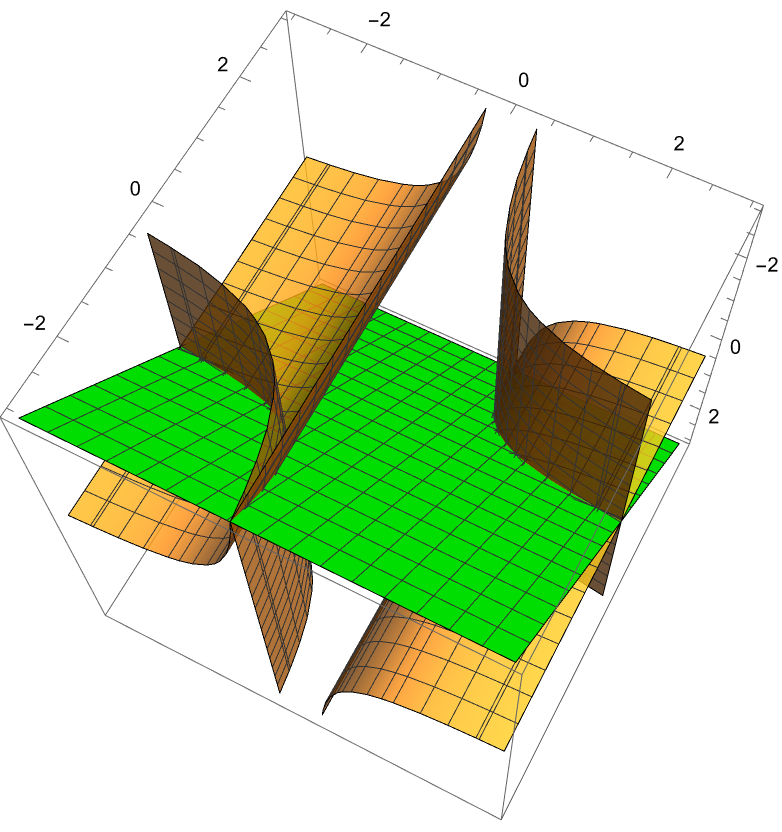
\includegraphics[width=1\linewidth]{12}
		\caption*{Each polynomial is a surface}
		\label{fig:12}
	\end{subfigure}
	\begin{subfigure}{0.5\textwidth}
		\centering
        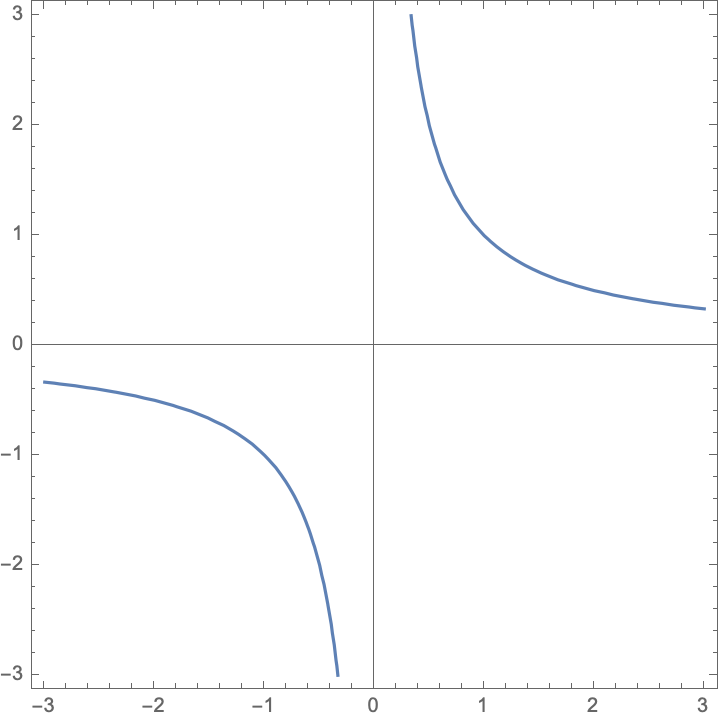
\includegraphics[width=1\linewidth]{13}
		\caption*{$V(f_1,f_2,y-z)$ is this curve}
		\label{fig:13}
		\end{subfigure}
	\end{figure}
 Project $\pi_1:\C^3\to\C^2$ with $(p_1,p_2,p_3)\mapsto (p_2,p_3)$ and show $\pi_1(V(f_1,f_2))=V(y-z)\backslash\{(0,0)\}$.

\end{ex}
\subsection{Elimination theory}
*There's something missing here*
\begin{thm}[Extension theorem]
	$I=\langle f_1,...,f_s\rangle\subseteq\C[x_1,...,x_m]$. Let $I_1=I\cap\C[x_1,...,x_m]$ we will write $f_i$ as
	$$
	f_i=c_i(x_1,...,x_m)x_1^\alpha+\text{forms of degree }<\alpha_1 \text{ wrt }x<
	$$
	such that $c_i\in\C[x_1,...,x_r]$ is non zero.\par
	If $(f_1,...,f_m)\in V_{\C^{m+1}}(I_1)\backslash V_{\C^{m+1}}(c_1,...c_s)$ then $\exists p_1\in \C$ such that $(p_1,...,p_m)\in C(I)$.
\end{thm}
\begin{thm}[Closure theorem]
	$V_{\C^{m-\ell}}(I_\ell)=\overline{\Pi_\ell(V_{\C^m}(I))}$
\end{thm}
\begin{thm}[Elimintation theorem]
	Let $G$ be a GB of $I$ with respect to $>_\lex$. Then, $G\cap\C[x_p,...,x_m]$ is a GB of $I$ with respect to $>_\lex$.
\end{thm}
\begin{lema}
	If $LM_{>_\lex}(f)\in\C[x_{\ell+1},...,x_m]$, then $f\in\C[x_{\ell+1},...,x_m]$
\end{lema}
\begin{prooof}
	Any monomial $x^\alpha$ involving a variable in $\{x_1,...,x_\ell\}$ sarisfies $x^\alpha>_\lex x^\beta$ for $x^\beta\in\C[x_{\ell+1},...,x_m]$. So, if $LM_{>_\lex}(f)$ does not involve $\{x_1,...,x_\ell\}$, no monomial in $\supp(p)$ involves $\{x_1,...,x_{\ell-1}\}$.
\end{prooof}
\begin{proof}
	Consider $f\in I_\ell$ as $G$ is GB, $\exists g\in G$ such that $LM_{>_\lex}(g)|LM_{>_\lex}(f)$ then $LM_{>_\lex}<_\lex LM_{>_\lex}(f)$, so by the lemma, $g\in\C[x_{\ell+1},...,x_m])\cap G$.
\end{proof}
\subsubsection{Saturation of ideals}
\begin{defn}
	Given ideals $I,J$ we define the saturation of $I$ with respect to $J$ as 
	$$
	(I:J^\infty)=\{f\in\C[x_1,...,x_m]|(\forall g\in J)(\exists k\in\N) g^k·f\in I\}
	$$
\end{defn}
\begin{ex}
	\begin{enumerate}
		\item $\langle x(x+1),y(x+1)\rangle:\langle x,y\rangle^\infty=\langle x+1\rangle$
		\item $\langle (x-y)xy,(x-y)^3x^4\rangle:\langle x-y\rangle^\infty=\langle xy,x^3\rangle$
	\end{enumerate}
\end{ex}
\begin{thm}
	$V(I:J^\infty)=\overline{V(I)V(J)}$
\end{thm}
\begin{thm}
	Let $I\subseteq\C[x_1,...,x_m]$ and $g\in\C[x_1,...,x_m]$. $I:\langle g\rangle^\infty=\langle I,1-tg\rangle_{\C[x_1,...,x_m,t]} \cap\C[x_1,...,x_m]$
\end{thm}
\begin{obs}
	$g\in\sqrt{I}\iff1\in\langle I,1-tg\rangle_{\C[x_1,...,x_m,t]}\iff(I:\langle g\rangle^\infty)\ni1$
\end{obs}
\begin{prop}
	$(I:(J_1+J_2)^\infty)=(I_J^\infty)\cap(I:J_2^\infty)$
\end{prop}
\begin{cor}
	If $J=\langle g_1,...,g_2\rangle$, then $(I:J^\infty)=\bigcap_{i=1}^s(I:\langle g_i\rangle^\infty)$
\end{cor}
\subsection{Exercises}
\begin{exer*}[1.2] Given a polynomial ring $R$ like $\C[y]$, prove there are two polynomials $A,B\in R[x]$ such that $\Res(f,g,x)=Ag+Bf$ such that $\deg _x(A)<\deg_x(g)$ and $\deg_x(B)<\deg_x(f)$. \textbf{Hint:} consider the adjugate matrix of the Sylvester matrix.\par
\begin{proof}[Solution]
    Recall our definition of the Sylvester matrix:
\begin{defn}[Resultant]
	Given $f(x,y)=\sum_{i=1}^m f_i(y)x^i \in\C[x,y]$ that is, $f\in\C[y]$, and $g=\sum_{i=1}^m g_i(y)x^i$. We define Sylvester matrix $\text{Sylv }(f,g,x)$.\\
	\begin{align*}
		\begin{pmatrix}f_m&0&...&0&g_m&0&...&0\\ 
			f_{m-1}&f_{m}&...&0&g_{m-1}&g_{m}&...&0\\
      &&...&&&&...&\\
			f_0 & f_1&...&f_m&g_0 & g_1&...&g_m\\
			0&f_0&...&f_{m-1}&0&g_0&...&g_{m-1}\\
         &&...&&&&...&\\
   			0&0&...&f_0&0&0&...&g_0\\
		\end{pmatrix}
	\end{align*}\par
	The resultant $Res(f,g,x)=\det \text{Sylv }(f,g,x)\in \C$.
 \end{defn}
Notice that for our excersie we need a more general definition: de degrees of $f$ and $g$ may be different. An attempt to write a general matrix is:
	\begin{align*}
		\begin{pmatrix}f_n&0&...&0&g_m&0&...&0\\ 
			f_{n-1}&f_{n}&...&0&g_{m-1}&g_{m}&...&0\\
      &&...&&&&...&\\
			f_{n-m} & f_1&...&f_m&g_? & g_1&...&g_m\\
   			f_{n-(m-1)} & f_1&...&f_{m-1}&g_? & g_1&...&g_m\\
			0&f_0&...&f_{?}&0&g_0&...&g_{m-1}\\
         &&...&&&&...&\\
   			0&0&...&f_0&0&0&...&g_0\\
		\end{pmatrix}
	\end{align*}\par	
 So maybe we take $n=2$, $m=1$. Then $f=f_2x^2+f_2x+f_0$ and $g=g_1x+g_0$, thus
 \begin{align*}\Sylv(f,g,x)=
     \begin{pmatrix}
         f_2&g_1&0\\
         f_1&g_0&g_1\\
         f_0&0&g_0
     \end{pmatrix}
 \end{align*}
Recall the formula $$\det(A)Id=A^*A$$
donde $A^*$ es la matriz adjunta. (unfinished)
\end{proof}
\end{exer*}
\newpage

%Here's should be differential algebra part.
\section{Differential Algebra}
\label{difalg1}
We'll use the team's paper \cite{falkensteiner2020fundamental}, François' short notes (sent to us) and long notes \cite{Francois}, and Sebastian's notes \cite{Sebastian}. Recall many ideas were first defined in \cite{kolchin1973differential} and \cite{ritt1950differential}.
\subsection{Differential polynomial rings and related notions}
\begin{defns}\leavevmode
\begin{itemize}
    \item An operator $\delta$ is called a \textbf{derivation operator} if $\delta(a+b)=\delta a+\delta b$ and $\delta(ab)=(\delta a)b+a\delta b$ for all elements $a,b$ in a ring.
    \item A \textbf{partial differential ring} is a pair $(R,D)$ consisting of a commutative ring with unity $R$ and a set $D=\{\delta_1,...,\delta_n\}$ of $m>1$ \textbf{derivations} wich act on $R$ and are pairwise commutative.
    \item We denote by $\Theta$ the free commutative monoid generated by $D$.
    \item Let $(R,D)$ be a partial differential ring and $x_1,...,x_n$ be $n$ \textbf{differential indeterminates}. The monoid $\Theta$ acts on the differential indeterminates giving an infinite set of \textbf{derivatives}.
    \item We denote by $R\{x_1,...x_,n\}$ the ring of polynomials with coefficients in $R$ and indeterminates wich are the derivatives. So for example:
    $$R\{x\}:= R[x,\dot{x},\ddot x,...]$$
    are polynomials in the infinite set of derivative indeterminates. We may also denote this set by $R[\Theta X]=R\{x_1,...,x_n\}$ where $X$ is the set of indeterminates.
    \item Then $(R\{x_1,...,x_n\},D)$ is a \textbf{differential polynomial ring}.
    \item A differential polynomial induces an evaluation map from $R^n$ to $R$. A \textbf{zero} or \textbf{solution} of $P\in R\{x_1,...,x_n1\}$ is an $n$-tuple $\varphi\in R^n$ such that $P(\varphi)=0$. For any $\Sigma\subseteq R\{x_1,...,x_n1\}$ we denote $\Sol\Sigma$ the set of solutions to every element of $\Sigma$
    \item A \textbf{differential ideal} is an ideal in this ring that is stable under the action of $\Theta$.
    \item A \textbf{perfect} differential ideal is an ideal that is equal to its radical.
    \item  If $\Sigma\subseteq R\{x_1,...,x_n1\}$ then $[\Sigma]$ is the ideal generated by $\Sigma$ and $\{\Sigma\}$ is the perfect differential ideal generated by $\Sigma$, defined as the intersection of all perfect differential ideals containing $\Sigma$.
\end{itemize}
\end{defns}
\begin{prop}
    For any $\Sigma\subseteq R\{x_1,...,x_n1\}$ there is a finite subset $\Phi\subset R^n$ such that $\Sol\Sigma=\Sol\Phi$.
\end{prop}
\subsection{Rankings}
\begin{defns}
    Let $Y=\{y_1,...,y_n\}$ be a set of differential inderetminates.
    \begin{itemize}
    \item A \textbf{ranking} is a total ordering on $\Theta Y$ such that for all derivative $u,v\in \Theta Y$ and all derivations $\theta \in \Theta$:
        \begin{itemize}[label=\textbullet]
            \item $v\leq\theta v$
            \item $v<w\implies \theta v<\theta w$
         \end{itemize} 
    \item The \textbf{leading derivative} of $p\in \mathcal F\{y_1,...,y_n\}$ is the highest derivative $v\in\Theta Y$ such that the degree of $p$ with respect to this derivative is positive, ie. $\deg (p,v)>0$.
    \item Let $d=\deg(p,v)$ with $v$ the leading derivative of $p$. Then $v^d$ is the \textbf{rank} of $p$.
    \item \textbf{Thm.} Raking is a well-ordering (every finite strictly descending sequence of derivatives is finite).
    \item The \textbf{initial} of $p$ is the leading coefficient in $p$ seen as a univariate polynomial in $v$.
    \item The \textbf{separant} of $p$ is the partial derivative of $p$ with respect to its leading derivative.
    \begin{itemize}[label=\leavevmode]
        \item So for example if $p=\dot u^2+u^3$ its leading derivative is $\dot u$. So separant$(p)=\frac{\partial p}{\partial \dot u}=2\dot u$ as $u^3$ is constant respect to $\dot u$.
    \end{itemize}
    \end{itemize}
\end{defns}
\subsection{Decomposition of Perfect Differential Ideals}
First recall:
\begin{defn}\leavevmode
    \begin{itemize}
        \item An ideal $\mathfrak p\subset R$ is \textbf{prime} if for all $a,b\in R$ we have $ab\in\mathfrak p\implies [a\in\mathfrak p$ or $b\in\mathfrak p]$.
        \item An ideal $\mathfrak q\subset R$ is \textbf{primary} if for all $a,b\in R$ we have $ab\in\mathfrak q\implies [a\in\mathfrak p$ or $\exists e\in\N, b^e\in\mathfrak q]$.
    \end{itemize}
\end{defn}

A representation of a perfect differential ideal $\mathfrak U$
$$
\mathfrak U=\mathfrak B_1\cup...\cup\mathfrak B_\varrho$$
is called \textbf{minimal} if for any different indices $1\leq i,j\leq\varrho$ we have $\mathfrak B_i\not\subset\mathfrak B_j$.
\begin{thm}[From Françoi's short notes]
    There exists a unique minimal representation of a perfect differential ideal $\mathfrak U$ as a finite intersection of prime differential ideals.
\end{thm}
\begin{thm}[From Fracnçoi's long notes. (Lasker-Noether Theorem)]
For every ideal $\mathfrak a\subset R$ is a finite minimal intersection of of primary ideals $$\mathfrak a=\mathfrak q_1\cap ...\cap \mathfrak q_r$$.\\ Such a \textbf{minimal primary decomposition} is not necessarily unique but, if $$\mathfrak a=\mathfrak q'_1\cap...\cap\mathfrak q_{r'}$$ is another minimal primary decomposition of $\mathfrak a$, then $r=r'$ and the 'set of the associated prime ideals $\mathfrak p_1,...,\mathfrak p_r$ of the two decompositions' is uniquely defined (that is, the $\mathfrak p_i$ are the associated \textit{prime} ideals of $\mathfrak a$, I think those from the last theorem).
    
\end{thm}
\subsection{Triangular sets and regular chains}
\textbf{(Here we pass from Françoi's long notes \cite{Francois} to Sebastian's notes \cite{Sebastian}.)}\par

Let us say for now that a \textbf{triangular set} is a set of polynomials $A=\{p_1,...,p_r\}$  with some properties related to their leading variables (or leading derivatives, as defined earlier). Define $I_A=i_1...i_r$ the product of the initial derivatives of the $p_i$.
\begin{defn}
    The ideal generated by the triangular set $A$ is denoted $$\mathfrak a=(A):I^\infty_A$$And we shall also consider $$(A):S_A^\infty\qquad\text{and}\qquad(A):H_A^\infty$$ where $S^\infty_A$ is the product of the separants of $A$ and $H_A^\infty$ is the product of the initials and the separants of $A$.
\end{defn}
\begin{thm}
    If $A$ is a triangular set, then $(A):S_A^\infty$ is radical.
\end{thm}
\begin{defn}
    Regular chain.
\end{defn}
\begin{thm}
For a given set of polynomials $\Sigma$ there are finitely many regular differential chains $A_1,...,A_\varrho$ such that $$\{\Sigma \}=[A_1]:H^\infty_{A_1}\cap...\cap [A_\varrho]:H^\infty_{A_\varrho}$$ is a decomposition of the perfect differential ideal $\{\Sigma\}$ as an intersection of perfect differential ideals. We may ``add $H_i^\infty$ as inequalities to the regular differential chains $A_i$".
\end{thm}
We shall call perfect differential ideals of the form $\mathfrak U=A:H^\infty_A$ given by single regular differential chains $A$ \textbf{characterizable ideals}.\par
Using the ``Thomas decomposition", we find there is a decomposition of the solution space
$$\Sol(\mathfrak U)=\dot\bigcup_{1,...,\varrho}\Sol(A_i)$$
\begin{thm}[Nullstellensatz]
    If $\mathfrak U\subsetneq \mathcal F\{u_1,...,u_n\}:=F\{\mathbf{u}\}$ is a radical differential ideal, then $\Sol(\mathfrak U)\neq\emptyset$ and $p$ is a polynomial that vanishes in $\Sol(\mathfrak U)$, then $p\in\mathfrak U$.
\end{thm}
\subsection{Zero testing}
\begin{defns}\leavevmode
\begin{itemize}
    \item Take a formal power series $u(x)\in\C[[x]] = \left\{ \sum_{i=0}^\infty a_i x^i : a_i \in \C \right\}$. We call $u(x)$ \textbf{differentially algebraic} if there is $p\in \mathcal F\{u\}\backslash\mathcal F$ such that $p(u(x))=0$.
    \item In this case we say $p$ is the \textbf{annihilator} of $u(x)$
    \item If $p$ can be chosen to be in $\mathcal F[u]\backslash\mathcal F$, that is, if $p$ doesn't involve any derivatives, we just say $u(x)$ is \textbf{algebraic}.
\end{itemize}
\end{defns}
So what is is this saying? Let $p$ be just $p=\dot u$, then $p(u(x)) = \dot u=\sum_{i=1}^\infty a_i \cdot i \cdot x^{i-1}$. All there's to it really is a differential equation: if $p$ annihilates $u(x)$, then we're just saying $\dot u=0$. Thus every $p\in \mathcal F\{u\}\backslash\mathcal F$ is really a differential equation which can be evaluated in formal power series. (Notice formal power series are \textit{not} the same as holomorphic functions in $\C$). So the roots of these polynomials are just the solutions of the differential equations. \textit{That's the whole idea}.\par
%In the course we'll see how to count the zeroes of a family of differential equations (a differential ideal) according to the decomposition given in the first sections. But let's continue for now.
\begin{prop}
    The set of differentially algebraic functions is a ring which is closed under composition, differentiation and division (if they are defined).
\end{prop}
The coefficients of a differentially algebraic function cannot be arbitrary:
\begin{prop}
    A formal power series $u(x)$ is differentially algebraic over $\mathcal F$ $\iff$ $\mathcal F\{u(x)\}$ has finite trascendence degree over $\mathcal F$.
\end{prop}
\begin{ex}
    $u(x)=1+\log(x)$ is differentially alebraic but not algebraic with annihiliator $p=x\dot u-1$. Now consider $q=\exp(u)-1$. Then $q(u(x))\neq0$ but $q(0+\log(x))=0$ \textit{Why?}
\end{ex}
\begin{obs}[Structural relation]
    $\text{prem}(q,A)=0\iff q\in\{A\}\iff\Sol(A)\subseteq\Sol(q)$
\end{obs}
\begin{ex}
\begin{align*}
        A&=\{p_1=u^2-x^3,p_2=v^5-x^3u\}\\
        q&=8u'^3-27u\\
        (u(x),v(x))&=(x^{3/2},x^{9/10})\text{ is a zero of }A\text{ and prem}(q,A)\neq0
\end{align*}
And now make a slight change in $p_2$:
\begin{align*}
        A&=\{p_1=u^2-x^3,p_2=v^{10}-x^9\}\\
        q&=8u'^3-27u\\
        (u(x),v(x))&=(x^{3/2},x^{9/10})\text{ is again a zero of }A\text{ and prem}(q,A)\neq0
\end{align*}
but in this second case we also have $q(u(x),v(x))=0$.
\end{ex}
So if the remainder was zero the we would already have an answer for the zero testing. If not, we are showing what to do.
\subsection{Root separation bound}
Take $p\in \mathcal F\{\mathbf{u}\}$ to be the anihilator of $u(x)$. Then $\rho\in\N$ called a \textbf{root separation bound} at $u(x)$ if it is the smallest number such that for every $v(x)\in\Sol(p)\backslash\{u(x)\}$, $\text{ord}(u(x)-v(x))>\rho$. This is like a smallest distance between all the solutions of $p$. (We are somehow trying to isolate roots so as to find solutions to differential equations.)

\begin{algorithm}[H]
\caption{ZeroTest($q$)}
	\SetKwInOut{Input}{Input}
	\SetKwInOut{Output}{Output}
	
	\Input{$u(x) \in \mathbb{C}[[x]]$ with annihilator $p \in \mathcal F\{u\}$ and $q \in \mathcal F\{u\}$}
	\Output{\textbf{true} if $q(u(x)) = 0$ and \textbf{false} otherwise}

 		\begin{enumerate}
 		    \item If $q \in \mathbb{C}[x]$, return $q = 0$
\item If ZeroTest$(Iq)$ then return ZeroTest$(\text{prem}(q,Iq))$
\item If ZeroTest$(Sq)$ then return ZeroTest$(\text{prem}(q,Sq))$
\item If $\text{prem}(q, p) \neq 0$ then return ZeroTest$(\text{prem}(q, p))$
 		\end{enumerate}
	\Return{$\text{ord}_x(q(u(x))) > 2\rho_{q,u(x)}$}\;
\end{algorithm}

\subsection{Counting solutions of differential equations}
Let $p\in\mathcal F\{u\}$. Where $p(u(x)) =0$ is of finite transcendence degree.
\begin{defns}[And an example]\leavevmode
\begin{itemize}
    \item     (Chat GPT). Let $L/K$ be a field extension, and let $\alpha$ be an element of $L$. The transcendence degree of $\alpha$ over $K$, denoted as $\text{trdeg}_K(\alpha)$, is the transcendence degree of the field extension $K(\alpha)/K$. It measures the number of algebraically independent elements in $K(\alpha)$ over $K$.
    
    \item     Let $\mathfrak U$ (for example, $\mathfrak U=(u^3,u,v)\subseteq \Q[u,v]$) be an algebraic prime ideal. Then $\dim \mathfrak U $ is defined as the transcendence degree of $\mathcal{F}(\mathbf{u})/\mathfrak U$. This is computed via Gröbner basis.

    \item The Hilbert Function is
    \begin{align*}
        \Omega_{\mathfrak U}:\N&\to\N\\
        \ell&\mapsto \dim(\mathcal F(\mathbf{u}_\ell/\mathfrak U_\ell)
    \end{align*}
    So in our example we have $\Omega_{\mathfrak U}(0)=1,\Omega_{\mathfrak U}(1)=3,\Omega_{\mathfrak U}(\ell)=\ell+3$ for $\ell\geq2$, so this is a polynomial in $\ell$.
\end{itemize}
\end{defns}
Computed the generic solutions of the system of differential equations given by
$$u_i(\mathbf{x})=u_i(x_1,...,x_m)=\sum c_{i,\theta}(x_1-\xi_1)^{e_1}...(x_m-\xi_m)^{e_m}$$
then derived algebraic condicions on the $c_{i,\theta}$ for the differential dimension: number of unspecified coefficientes, differential counting, number of possible chrees (?).\par
So let $\mathfrak U\subseteq \mathcal F\{\mathbf{u}\}$ be a differential ideal. Usually require that $\mathfrak U$ is given via a regular differential chain, that is $\mathfrak U=[A]$. So now we have a \textbf{differential dimension function}
    \begin{align*}
        \Omega_{\mathfrak U}:\N&\to\N\\
        \ell&\mapsto \dim(\mathcal F(\mathbf{u}_{\leq\ell}/\mathfrak U_{\leq\ell})
    \end{align*}
Where $\mathfrak U_{\leq\ell}$ are the elements in $\mathfrak U$ of order less or equal to $\ell$.
\begin{prop}
    Is $\mathfrak U$ is a characterizable differential ideal with corresponding regular differential chain $A$, and set of leading derivatives $\text{lead}(A)$, then for every $\ell\in\N\cup\{\infty\}$ we have
    $$\Theta\{\mathbf{u}\}_{\leq\ell}\backslash\Theta\text{lead}(A)_{\leq\ell}=\dim(\mathcal \{\mathbf{u}\}/\mathfrak U_{\leq\ell}$$
\end{prop}
\begin{ex}
    The Burger's equation $p = u_{x_1,x_1} - u_{x_2} - 2u u_{x_1}$ defines a regular differential chain (w.r.t. any ranking). We shall obtain that $\omega_{\{p\}}(\ell) = 2\ell + 1$.
\end{ex}
So whenever we have out assumption that $\mathfrak U=[A]$ then the counting function will be a polynomial in $\ell$.
\begin{thm}\leavevmode
    \begin{enumerate}
        \item There exists a numerical polynomial $\omega_{\mathfrak U} \in \mathbb{Q}[\ell]$, called the \textbf{differential dimension }polynomial, with $\Omega_{\mathfrak U}(\ell) = \omega_U(l)$ for sufficiently large $\ell \in \mathbb{N}$.
        \item This polynomial is of degree less os equal to $n$ and can be written as $\omega_{\mathfrak U}(\ell)=\sum_{i=1}^ma_i{\ell+i\choose i}$ for some $a_i\in\Z$.
        \item $a_m$ is the \textbf{differential dimension}
        \item If $\mathfrak B=[B]$ is another characterizable ideal of $\mathcal F\{\mathbf{u}\}$ with respect to the same ranking. It $\mathfrak U\subseteq\mathfrak B$, then $\omega_{\mathfrak U}\leq\omega_{\mathfrak B}$. Moreover, $\mathfrak U=\mathfrak B$ if and only if
        \begin{itemize}
            \item $\omega_{\mathfrak U}=\omega_{\mathfrak B}$
            \item The set of leaders of the corresponding regular chains are the same.
            \item The equations have the same degree.
        \end{itemize}
    \end{enumerate}
\end{thm}
Let us make a super simple example
\begin{ex}
    Take $p=u_{x_1}=0$ with $u(x_1,x_2)=\sum c_{ij}x^i_1x^j_2$. So
    $$\frac{\partial}{\partial x_1}(u(x_1,x_2))=\sum c_{ij}ix^{i-1}_1x^j_2=0$$
    and here $c_{ij}=0\forall i>0, j\in\N$. Then $c_{0j},...$ are free coefficients for all $j\in\N$.
\end{ex}
\subsection{Respresentation of differential equations}
Algebraic varieties are the zero sets of polynomials, that, as geomtric objects, they can be sometimes represented with a parametrization. We attempt to do this for differential system with what we shall call \textbf{realizations}.
\paragraph{Algebraic case}
\begin{itemize}
    \item     $\mathbb V(p)$ has a parametrization if and only iff genus is zero. For higher genus we might glue local parametrizations.
    \item For $p\in\Q[u_1,...,u_n]$ there exists and algorith for deciding the existence of a rational parametrization of $\mathbb V(p)$ in the case of $n=2,3$, and it can compute it.
\end{itemize}
\paragraph{Differential case}
Now take $\{p_1,...,p_r\}\in\mathcal F\{u_1,...,u_n\}$. An \textbf{explicit representation} of these polynomials is a dynamical system
    $$\begin{cases}
        \mathbf{\dot t=f(t,y)}\\
        \mathbf{ u=g(t,y)}
    \end{cases}$$
    where everything is bold because they are vectors. So $\mathbf{f,g}$ are rational functions in $\mathbf{t,y}$.\par
Let us nos consider the problem of going from a realization to a implicit representation.
\begin{align*}
    \dot{\mathbf{t}}\cdot Q-\mathbf F,\qquad \mathbf u \cdot Q-\mathbf G\\
    \frac{\mathbf F}{Q}=f_i,\qquad\frac{\mathbf G}{Q}=g_i\\
    \text{(unfinished)}\qquad
\end{align*}
Anyway, to go back to a realization, it is a necesassary condition that $\mathbb V(p_1,...,p_r)$ is a rational variety.\par
So let us consider a polynomial $p\in \Q\{ x, y\}=\Q[u,...,u^{(N)},y,...,y^{(N)}$ and $\mathbf a(t)\in\Q(y)(t)\times\Q(y,...,y^{(N)})(\mathbf t)^N$ a rational parametrization of a hypersurface $\mathbb V(p)$. And eventually conclude that
$$
\mathbb V(p) \text{ is rational}\iff p\text{ is realizable}$$
\subsection{Finding solutions}
\subsubsection{Rational solutions}
We look for solutions like
$$u(x)=\frac{c_0+c_1x+...+c_r}{d_0+d_1x+...+d_kx^k}
$$ for $r,k\in\N$.\par
We may have $p_1,...,p_m\in\Q(\mathbf x)\{\mathbf{u}\}$ and assume that $\mathbb V(p_1,...,p_m)$ is rational. Now we may take a rational parametrization $\mathcal P$ of it, so there is a dynamical system such that
\begin{align*}
    (1)&\qquad\mathcal p(\mathbf t(\mathbf x))=\mathbf u(\mathbf (x))\\
    (2)&\qquad \mathbf u(\mathbf x))\not\in\img(\mathcal P)
\end{align*}
for some $\mathbf t(\mathbf x))\in\Q(\mathbf x)^N$.
We develop necessary and sufficient conditions for finding solutions of rational first order differential equations:
\begin{thm}
    For $p\in\Q[u,u']$, the equation $p=0$ has a rational solution, then $\mathbb V(p)$ is a rational algebraic variety.\par
    If $\mathcal P=(p_1,p_2)$ is a rational parametrization of $\mathbb V(p)$, then $t=\frac{p_2}{p_1}$ has a rational solution if and only if $\exists a,b\in\Q$ such that $\frac{p_2}{p'_1}=b·(t-a)^2$. In this case, $u(s)=p_1(t(x+c))$ is a ratinoal generic solution.
\end{thm}
\begin{ex}
    Let $p=\dot u^3+4\dot u^2+ (27u^2+4)\dot u+27u^4+4u^2$ and $\mathcal P=(216t^3+6t,-3888t^4-36t^2)$. So we have
    \begin{align*}p_2/p'_1&=-6t^2=t'\\t(x)&=\frac{1}{6(x+c)}\\&\implies u(x)=p_1(t(x))=\frac{(x+c)^2+1}{(x+2)^2}\end{align*}
\end{ex}
\subsubsection{Algebraic solutions}
We now consider $u(x)$ as a zero of $q(x,u)$ for $p\in\Q[u,u']$. And we must
\begin{itemize}
    \item Compute a local solution $u(x)$.
    \item Guess/check whether $u(x)$ is algebraic.
\end{itemize}
\begin{thm}
    If there exists and algebraic solution of $p=0$, then all local solutions of $p=0$ are algebraic. If $q(x,u)$ is the minimal polynomial associated, then $$\deg_x(q)=\deg_{u'}(p),\quad\deg_u(q)\leq\deg_u(p)+\deg_{u'}(p)$$
\end{thm}
\begin{ex}
    Take $p=u^4+3u'$ and $\mathcal P=(t,-t^4/3)$ so that $p_2/p'_1=\frac{-t^4/3}{t}$ and there's no rational solutions. Then, for the initial value $u(0)=1$ and $u'(0)=-1/4$. Eventually we arrive to $q=xu^3-1$
\end{ex}
\subsubsection{Local solutions}
Take $p=\Q[u,u']$ so that $\mathbb V(p)$ always admits a local parametrization $\mathcal P\in\Q((t))^2\backslash\Q^2$ which can be computed using the Poisseaux expansion as was shown in Fuensanta's course.
\begin{thm}
    Take a local parametrization $o:=\mathcal P=(p_1,p_2)$ of $\mathbb V(p)$. If $\text{ord}(p_1-p_2(0)-\text{ord}(p_2)>0$ then there exist exactly $o$-many formal power solutions of $p$ with initial value $u(0)=p_1(o),u0(0)=p_2(o)$ and the corresponding branch (we must always choose a branch).
\end{thm}
\begin{ex}
    $p=((u'-1)^2+u^2)^3-4(u'-1)^2u^2=0$ and $(p_1,p_2)=(t^2,1+\sqrt{2+}\frac{3t^3}{4\sqrt{2}}+...)$\par
We shall obtain that $u(x)=x\pm\frac{2\sqrt2x^{3/2}}{3}+...$
\begin{figure}[H]
    \centering
    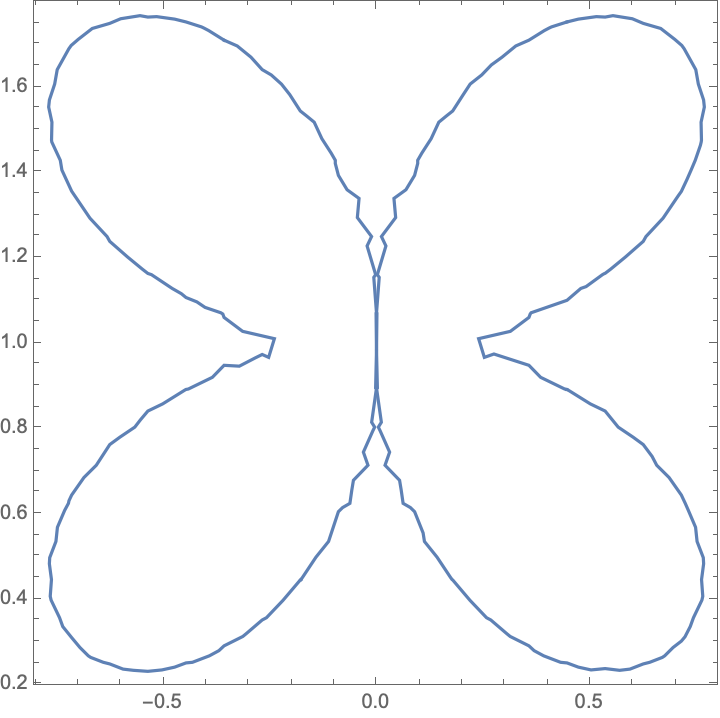
\includegraphics[width=0.5\textwidth]{Notas2/LastFig.png}
\end{figure}
\end{ex}
\newpage
\subsection{(Extra) Another view of Tropical Geometry}
Now that we've read some of \cite{falkensteiner2020fundamental}, let us define the following ideas that are related to the \hyperref[tropgeom]{Tropical Geometry course}:
\begin{defn}\leavevmode
\begin{itemize}
    \item For $m\geq1$ denote by $\mathcal P(\Z_{\geq0}^m)$ the idempotent semiring whose elements are the subsets of $\Z_{\geq0}^m$ equipped with the union $X\cup Y$ as sum and the Minkowsky sum $X+Y=\{x+y:x\in X, y\in Y\}$ as product. (Here $nX$ denotes the sum of $X$ $n$ times). This structure is the \textbf{semirring of supports}.
    \item For an element $X\in\mathcal P(\Z_{\geq0}^m)$, we define the \textbf{Newton polygon} $\mathcal N(X)\subseteq \R^m_{\geq0}$ as the convex hull of $X+\Z_{\geq0}^m$. It looks like this is all the right-up translates of the set $X$.
    \item Now we call $x\in X$ a vertex if it is in the left-down boundary of the Newton polygon, that is, is $x\notin X\backslash \{x\}$. And we denote $\Ver X$ the set of vertices of $X$.
\end{itemize}
\end{defn}
\begin{lema}
    If two subsets $S,T\in\mathcal P(\Z_{\geq0}^m)$ have the same Newton polygon, then their vertices sets are the same.
\end{lema}
\begin{lema}
    The Newton polygon of the vertex set of $X$ is the same as the Newton polygon of $X$, that is, for any $X\in\mathcal P(\Z_{\geq0}^m)$, $\mathcal{N}(X)=\mathcal{N}(\Ver(X))$.
\end{lema}
\begin{cor}
\label{dfcor1}
    For any $X,Y\in\mathcal P(\Z_{\geq0}^m)$, we have $\Ver(X)=\Ver(Y)\iff\mathcal{N}(X)=\mathcal{N}(Y)$
\end{cor}
 \begin{figure}[H]
		\centering
		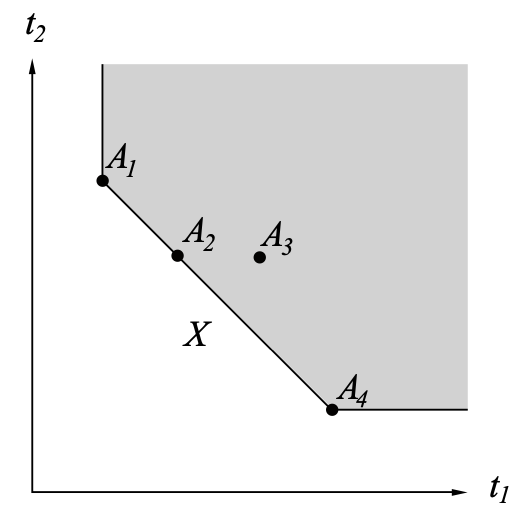
\includegraphics[width=0.5\linewidth]{df1}
		\caption*{Example of a Newton polygon}
		\label{fig:4}
	\end{figure}
\begin{defn}\leavevmode
\label{difalgtrop}
    \begin{itemize}
    \item Define the map $\Ver:\mathcal P(\Z_{\geq0}^m)\to\mathcal P(\Z_{\geq0}^m)$, which satisfies, by the Corollary, that $\Ver^2=\Ver$.
    \item Denote by $\T[[t_1,...,t_m]]$ the image of the operator $\Ver$, whose elements we call \textbf{vertex sets} or \textbf{tropical formal power series}. We define for $S,T\in \T[[t_1,...,t_m]]$,
    $$
    S\oplus T=\Ver(S\cup T)\qquad\text{and}\qquad S\odot T=\Ver(S+T)
    $$
    \end{itemize}
\end{defn}
\subsection{Problems on algebraic differential equations}
\begin{enumerate}
    \item Finding rational algebraic $d$ finite solutions (solutions of algebraic equations with polynomial coefficients) of alebraic differential equations.\par
    We know some things about the support (the zeroes) the functions involved in these equations. Use this knowledge to say something about possible solutions. This is known only for linear differential equations—we should be able to work on other types of differential equations.
    \item Which eliminations and combinations could be used for simplifiyng differential systems? Maybe something from tropical algebraic geometry could help!\par
    \item What we used for the computations of the solutions in 1. can also be used for computing simplifications of algebraic systems. Speed up computations.
    \item Prove DL (Denef and Lipsitz) Thm 3.1.
\end{enumerate}
\subsection{Exercises}
\begin{exer*}
    Apply the Zero-Testing algorithm to $u(x)=\sqrt{1+x}$ and $q$ for checking whether $q(u(x))=0$.
    \begin{enumerate}[label=\alph*)]
        \item $q=2uu'-1$
        \item $q=2uu'-1+x^{10}/10^{10}$
        \item $q=(2uu'-1)u''^2-xu+1$
    \end{enumerate}
\end{exer*}
\begin{proof}[Solution]
    Let us recall the Zero-Testing algorithm:
    \begin{algorithm}[H]
\caption{ZeroTest($q$)}
	\SetKwInOut{Input}{Input}
	\SetKwInOut{Output}{Output}
	
	\Input{$u(x) \in \mathbb{C}[[x]]$ with annihilator $p \in \mathcal F\{u\}$ and $q \in \mathcal F\{u\}$}
	\Output{\textbf{true} if $q(u(x)) = 0$ and \textbf{false} otherwise}

 		\begin{enumerate}
 		    \item If $q \in \mathbb{C}[x]$, return $q = 0$
\item If ZeroTest$(Iq)$ then return ZeroTest$(\text{prem}(q,Iq))$
\item If ZeroTest$(Sq)$ then return ZeroTest$(\text{prem}(q,Sq))$
\item If $\text{prem}(q, p) \neq 0$ then return ZeroTest$(\text{prem}(q, p))$
 		\end{enumerate}
	\Return{ord$_x(q(u(x))) > 2\rho_{q,u(x)}$}\;
\end{algorithm}
\begin{enumerate}[label=\alph*)]
    \item We have: $q \not\in\C[x]$, so we find $I_q=2u\not\in\C[x]$. So then we go on to find $S_q=I_q=2u\not\in\C[x]$. Now we must find the annihilator: $p=u^2-1-x$. Which has derivative $2uu'-1=q$, so that $\text{prem}(q,p)=0$, and we go to the last line of the algorithm, which happens to be \textbf{true}. Of course: $q(u(x))=2\sqrt{1+x}(1/2)(1+x)^{-1/2}-1=0$.
    \item Again $q \not\in\C[x]$, $I_q=2u\not\in\C[x]$ and also $S_q=I_q=2u\not\in\C[x]$. We have the same annihilator $p=u^2-1-x$ with has derivative $2uu'-1=q$. But how to calculate $\text{prem}(p,q)$?
\end{enumerate}
\end{proof}
\newpage
\section{Tropical Differential Algebra}
Let us consider a system of differential equations in $\R^4$:
\begin{align*}
\begin{cases}
	\frac{\partial y_1}{\partial t}&=\frac{1}{1200}y_1(t)+\frac{1}{500}y_2(t)+\frac{1}{500}y_3(t)\\
	\frac{\partial y_2}{\partial t}&=\frac{1}{1500}y_1(t)-\frac{1}{1000}y_2(t)+\frac{1}{1000}y_3(t)+\frac{1}{1000}y_4(t)\\
	\frac{\partial y_3}{\partial t}&=-\frac{1}{1000}y_1(t)-\frac{1}{500}y_2(t)+\frac{1}{500}y_3(t)+\frac{1}{1000}y_4(t)\\
 	\frac{\partial y_4}{\partial t}&=\frac{1}{1000}y_1(t)-\frac{1}{1000}y_3(t)\\
\end{cases}
\end{align*}
Where $y_i\in\mathcal C^1(\R^4)$. We can rewrite this as
\begin{align*}
\frac{{d\mathbf{y}}}{{dt}} &= \mathbf{A}\mathbf{y}
\end{align*}
That is,
\begin{align*}
\begin{pmatrix}
\frac{\partial y_1}{\partial t} \\
\frac{\partial y_2}{\partial t} \\
\frac{\partial y_3}{\partial t} \\
\frac{\partial y_4}{\partial t} \\
\end{pmatrix}=
\begin{pmatrix}
\frac{1}{1200} & \frac{1}{500} & \frac{1}{500} & 0 \\
\frac{1}{1500} & -\frac{1}{1000} & \frac{1}{1000} & \frac{1}{1000} \\
-\frac{1}{1000} & -\frac{1}{500} & \frac{1}{500} & \frac{1}{1000} \\
\frac{1}{1000} & 0 & -\frac{1}{1000} & 0 \\
\end{pmatrix}
\begin{pmatrix}
y_1 \\
y_2 \\
y_3 \\
y_4 \\
\end{pmatrix}
\end{align*}
It turns out $\mathbf{A}$ is diagonalizable, and the system can be converted to
\begin{align*}
\begin{pmatrix}
\frac{\partial x_1}{\partial t} \\
\frac{\partial x_2}{\partial t} \\
\frac{\partial x_3}{\partial t} \\
\frac{\partial x_4}{\partial t} \\
\end{pmatrix}=
\begin{pmatrix}
0.001&0 & 0& 0 \\
0& -0.001 & 0&0\\
0&0 & 0.001& 0\\
0& 0 & 0& -0.001 \\
\end{pmatrix}
\begin{pmatrix}
x_1 \\
x_2 \\
x_3 \\
x_4 \\
\end{pmatrix}
\end{align*}
That is,
\begin{align*}
\begin{cases}
	\frac{\partial x_1}{\partial t}&=0.001x_1(t)\\
	\frac{\partial x_2}{\partial t}&=0.001x_2(t)\\
	\frac{\partial x_3}{\partial t}&=-0.001x_3(t)\\
 	\frac{\partial x_4}{\partial t}&=-0.001x_4(t)\\
\end{cases}
\end{align*}
And has solution
\begin{align*}
    \begin{pmatrix}
x_1 \\
x_2 \\
x_3 \\
x_4 \\
\end{pmatrix}=
\begin{pmatrix}
x_1(0)e^{0.001t} \\
x_2(0)e^{0.001t} \\
x_3(0)e^{-0.001t} \\
x_4(0)e^{-0.001t} \\
\end{pmatrix}
\end{align*}
Where the exponents here are the eigenvalues.\par
Now let us choose initial conditions $x_1(0)=x_2(0)=x_3(0)=x_4(0)=1/2$.\par
So now we can change back to the original variables using the matrix made up of the eigenvectors:
\begin{align*}
    \begin{pmatrix}
y_1 \\
y_2 \\
y_3 \\
y_4 \\
\end{pmatrix}=
\begin{pmatrix}
1 & 1 & -1 & -1 \\
0 & 1 & 0 & 1 \\
1 & 0 & 0 & -1 \\
0 & 1 & 1 & 0 \\
\end{pmatrix}
\begin{pmatrix}
\frac{1}{2}e^{0.001t} \\
\frac{1}{2}e^{0.001t} \\
\frac{1}{2}e^{-0.001t} \\
\frac{1}{2}e^{-0.001t} \\
\end{pmatrix}
=
\begin{pmatrix}
\frac{1}{2}e^{0.001t} + \frac{1}{2}e^{0.001t} - \frac{1}{2}e^{-0.001t} - \frac{1}{2}e^{-0.001t} \\
\frac{1}{2}e^{0.001t} + \frac{1}{2}e^{-0.001t} \\
\frac{1}{2}e^{0.001t} - \frac{1}{2}e^{-0.001t} \\
\frac{1}{2}e^{0.001t} + \frac{1}{2}e^{0.001t} + \frac{1}{2}e^{-0.001t} \\
\end{pmatrix}
\end{align*}
We now ask two questions:
\begin{question}
    \item Is is to possible to tell apart between complex systems with feedbacks that create periodic solutions and the ones that do not have them through the classification of combinatoric objects in $\mathbb B[[t_1,t_2,...,t_n]]$? (Here $\mathbb B$ is a Boolean field so coefficients are 0's and 1's).
    \end{question}
So maybe there's a way to make a solution like
\begin{align*}
    \begin{pmatrix}
y_1 \\
y_2 \\
y_3 \\
y_4 \\
\end{pmatrix}=
\begin{pmatrix}
\frac{1}{2}e^{0.001t} + \frac{1}{2}e^{0.001t} - \frac{1}{2}e^{-0.001t} - \frac{1}{2}e^{-0.001t} \\
\frac{1}{2}e^{0.001t} + \frac{1}{2}e^{-0.001t} \\
\frac{1}{2}e^{0.001t} - \frac{1}{2}e^{-0.001t} \\
\frac{1}{2}e^{0.001t} + \frac{1}{2}e^{0.001t} + \frac{1}{2}e^{-0.001t} \\
\end{pmatrix}
\end{align*}
Into a combinatorial object like 
$$\begin{pmatrix}
1&0 & 1& 0 \\
0& 1 & 0&0\\
0&0 & 1& 0\\
0& 1 & 0& 1 \\
\end{pmatrix}$$
(number choices here are random). So its a matrix in $\mathbb B$.
\begin{question}\leavevmode Are there subgroups of $\text{Aut}(\mathbb{D}^2)$ such that their combinatorial objects are generated by a non tropical vector?\par
    Are there new properties on gradient flows over hyperbolic compact manifolds $\mathbb D^2/\text{Trop}(G)?$
    \end{question}
    So take a function $\omega:B^k_0\subseteq\C\to\C$ with $R=|z_0|$. And a nonlinear (but not complicated) differential equation
    \begin{align*}\frac{\partial \omega}{\partial z}&=\frac{\alpha}{c}\omega^2\\\omega(0)&=\beta+\frac{\alpha}{c}\frac{1}{z_0}\\\omega(z)&=\beta+\frac{\alpha}{c}\frac{1}{z-z_0}=\beta+\frac{\alpha}{c}\sum_{i=0}^\infty\frac{1}{z_0^{(i)}}z^i\end{align*}
    and recall $\text{Aut}(\mathbb D^2)=\{\frac{az+\bar c}{cz+\bar u}:|a|^2-|c|^2=1\}$
\subsection{Tropical Differential Algebraic Geometry}
    Let $k$ be a field of characteristic 0 and $m,n\in\N$. Define $$k_{m,n}=k[[t_1,...,t_m]][x_i,J:1\leq i\leq n, J\in\N^m]$$ to be a ring inspired in $\mathcal F\{\mathbf{u}\}$ which had $m$ variables $u_1,...,u_m$ and infinite derivatives. Also define the monoid $\Theta\cong\N^m=\langle \frac{\partial}{\partial t_1},...,\frac{\partial}{\partial t_m}\rangle$, and keep in mind the notation $\frac{\partial^{|J|}}{\partial t_1^{j_1}...\partial t_m^{j_m}}$ for $J=(j_1,...,j_m)\in\N^m$.\par
    Then $\Theta$ acts on $k_{m,n}$ by taking derivations of the functions. We shall work in the pair formed by our ring and this action, that is $(k_{m,n},\Theta:\N^m\times k_{m,n}\to k_{m,n})$.\par
    Define a differential equation $E$ to be \textbf{algebraic} if there exists $p\in k_{m,n}$ such that $V(p)\cong \Sol(E)=\{\varphi\in k[[t]]:p(\varphi)=0\}$. Let us arrive to tropical geometry from here.
\subsection{Twisted evaluation actions}
This is a map $ev_{P,\Theta}:k[\![ t_1,...,t_m]\!]^n\to S[\![ t_1,...,t_m]\!]$ for $P\in S_{m,n}$.
\begin{ex}
    Take the system $P\in\C_{2,1}$ with $$\begin{cases}P=tx_{(1,0)}+ux_{(0,1)}+(t^2+u^3)\\ E=t\frac{\partial \varphi}{\partial t}+u\frac{\partial \varphi}{\partial t}+(t^2+u^3)\end{cases}$$ so that by choosing
    \begin{align*}
        \varphi=t^2+t^1u+u^3\in\mathbb B[[t,u]]\\
        \frac{\partial\varphi}{\partial t}=t+u\\
        \frac{\partial\varphi}{\partial u}=t+u^2
    \end{align*}
    we get
    \begin{align*}ev_{(P,\Theta)}(\varphi)&=t(t+u)+u(t+u^2)+(t^2+u^3)\\&=(t^2+tu)+(tu+u^3)+t^2+u^3\\&=t^2+tu+u^3\end{align*}with $\varphi\in\C[[t,u]]$.\par
\end{ex}
   \begin{obs}
       Although we'd like to define $\varphi\in\mathbb B[\![ t,u]\!]$ to be a solution of $P\in\mathbb B_{2,1}$ is $P(\varphi)=0$, this will not work. Why?
   \end{obs}
    
    %Now consider a system of differential equations $\Sigma=\{E_1=...=E_s=0\}$ so that $\Sol(\Sigma)=\{\varphi\in\C[[t,u]]:E_i(\varphi)=0\forall i\}$.\parSo, what is the structure of $\Sol(\Sigma)$. Consider $\varphi\in\C[[t,u]]$ expressed as $\varphi=\sum a_{ij}x^iy^j$ and its support. Now we might as well consider the support of the whole solution set of a certain system $\Sigma$, that is $\supp(\Sol(\Sigma))$.
\subsection{Combinatorics}
Consider an operation $\mathbb V:\mathbb B[\![t,u]\!]\to\mathbb B[\![t,u]\!]$ that takes the Newton Polygon of a series and gives back the polynomial determined by the points in the boundary of the Newton Polygon. This is called the \textbf{vertex polynomial}. Now consider:
$$\begin{tikzcd}
\mathbb B[\![ t,u]\!] \arrow{r}[above]{\mathbb V}\arrow{dr} & \mathbb B[\![ t,u]\!] \\
&(\mathbb{VB}[t,u],\oplus,\odot)\arrow[hookrightarrow]{u} 
\end{tikzcd}$$
So it turns out we have a semirring $(\mathbb{VB}[t,u],\oplus,\odot)$.
\begin{defn}
    Let $a_1\oplus...\oplus a_k=a$ be a sum in $\mathbb{VB}[t,u]$. This sum \textbf{vanishes tropically} if $\forall(i,j)\in a$ there exist $\alpha\neq\beta$ such that $(i,j)\in a_\alpha,a_\beta$.
\end{defn}
\begin{ex*}[\textbf{ 30 Continued}]
    It turns out this example vanishes tropically. This example wasn't easy to find.
\end{ex*}
\begin{lema}
    If $\varphi\in\Sol(p)$, then $\supp(\varphi)\in\Sol(\supp(p))$.
\end{lema}
Which is easy to prove. And then we have:
\begin{thm}
    For an ideal $[\Sigma]\subset K_{m,n}$ with $m,n\geq1$, $\Sol(p_1,...,p_s)=\bigcap_{p\in[\Sigma]}\Sol(\supp(p))$
\end{thm}
Take a look at the school's poster:\par
\begin{figure}[H]\centering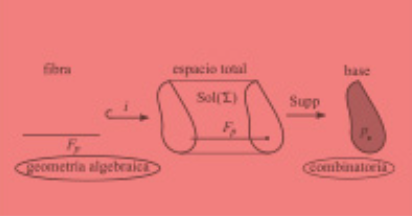
\includegraphics{Notas2/poster.png}\end{figure}
So that combinatorial objects given by the $\supp$ map give us information on the solutions of differential equations.
\begin{obs}
    Unlike notions of tropical convexity, tropical linear spaces are correctly defined using matriods. There is a relationship between matriods and tropical algebraic varieties that leads to visual figures.
\end{obs}

\subsection{An application of the lema}
Let's go for a theorem.
\begin{defn}[Circuits]
    Take $E\neq\emptyset$ and $\mathcal C\subset \mathcal P(E)$ such that
    \begin{itemize}
        \item $\emptyset\notin\mathcal C$.
        \item $S,T\in\mathcal C\implies S\not\subset T$ and $T\not\subset S$
    \end{itemize}
\end{defn}
\begin{defn}[Scruls]
    It's a free semigroup on circuits. $\mathcal S=\{C_1\cup C_2\cup C_3\cup...,\bigcup_{i\in I}\mathcal C_i\neq\emptyset, \mathcal C\in \mathcal S \text{ s.t. }\mathcal C\text{ is maximal}\}$
\end{defn}
\begin{thm}[A.L.S.G.]
    Let $W\subset K^E$ be a vector space with $E$ infinite uncountable and $\dim W<\infty$. Then
    $$\{\supp(v):v\in W\}\subset \mathcal P(E)$$
    is a matroid of scruls.
\end{thm}
So let $\Sigma\subset K_{m,n}$ be a h.s.l.d.e. such that $\dim\Sol(\Sigma)<\infty\implies\supp(\Sol(\Sigma))\subseteq\mathbb B[t_1,...,t_m]^n$. And we may consider the map
$$\mathbb B[t_1,...,t_m]\to\mathbb B[t_1,...,t_m,t_n,....,t_{nm}]$$
\begin{obs}[s]\leavevmode
\begin{itemize}
    \item It would be nice to have a scheme theory on tropical fields so as to have better geometry.
    \item We are still looking for applications of this technology.
    \item \textit{Don't we lose too much (qualitative) information when we booleanize differential equations?} Tropical geometry is ``made to lose" information. How much of it can we recover?
\end{itemize}
\end{obs}
\subsection{Exercises}
\begin{exer*}[4.1 (b)]
    We attempt to show that the sum of two polynomials is not equal to the union of each vertex set. Recall a vertex polynomial is a set of points in convex position.
\end{exer*}
\begin{exer*}[4.2]
    Consider $a=t^2u^3+t^3u+t^5=\{(2,3),(3,1),(5,0)\}$ and $b=u^4+tu^3+t^4u^2=\{(0,4),(1,3),(4,2)\}$ in $\mathbb B [\![t,u]\!]$.
    \begin{enumerate}[label=(\arabic*)]
        \item Show that $a$ and $b$ are vertex polynomials.
        \item Compute $a\oplus b$ and $a\odot b$ and show that the inclusion $a\oplus b\subset V(a)+V(b)$ is proper.
    \end{enumerate}
    \begin{proof}[Solution]
        \begin{enumerate}[label=(\arabic*)]
            \item \leavevmode\\
            \begin{figure}[H]
            \begin{subfigure}{0.5\textwidth}
                \centering
                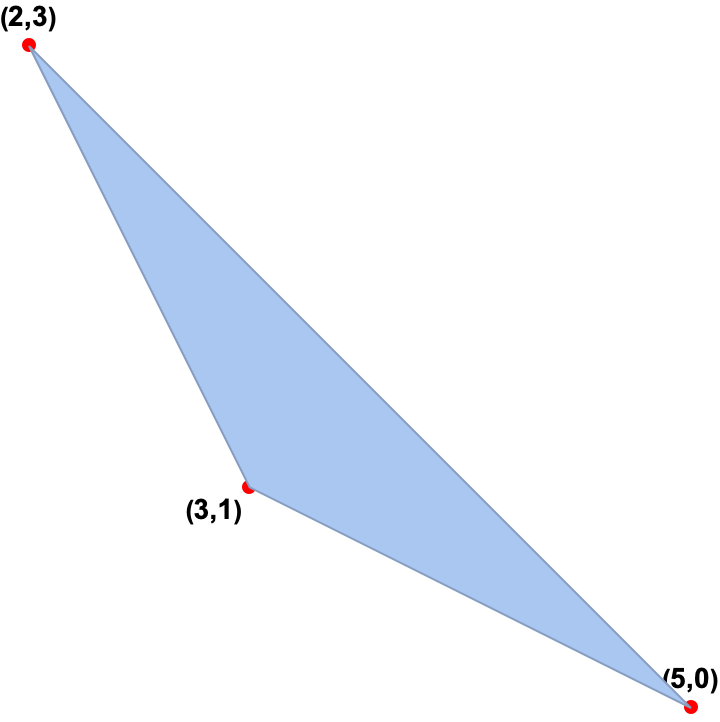
\includegraphics[width=0.9\linewidth]{Notas2/vertpoly1.png}
                \caption*{$a$}
            \end{subfigure}
            \begin{subfigure}{0.5\textwidth}
                \centering
                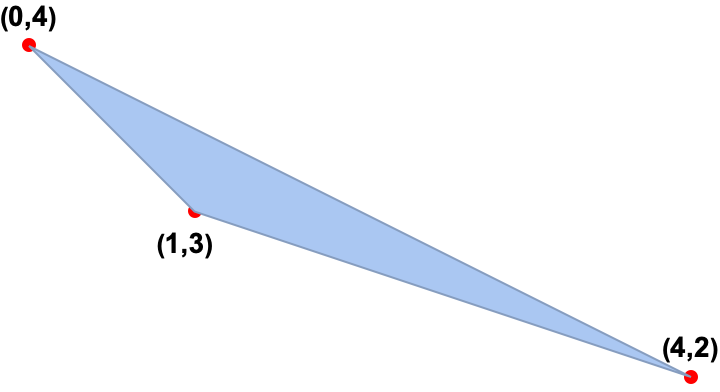
\includegraphics[width=0.9\linewidth]{Notas2/vertpoly2.png}
                \caption*{$b$}
            \end{subfigure}
            \end{figure}
    \item We have $a\oplus b=V(a+b)$ and $a\odot b=V(ab)$ with the operations of $\mathbb B[\![t,u]\!]$. So $a+b=t^2u^3+t^3u+t^5+u^4+tu^3+t^4u^2=$ (unfinished).
\end{enumerate}
\end{proof}
\end{exer*}
\newpage



\section{Newton's Method}
(See \cite{casas2019algebraic})\par
We will study Newton's method to parametrize algebraic curves, published in 1671. So let us start with a curve defined to be the zeroes of some function $f(x,y)=0$. We wonder if it is possible to make $y$ a function of $x$ so as to parametrize the curve.\par
Let us agree that $f(0,0)=0$ translating if necessary. Using the Implicit Function Theorem, we know that if $\frac{\partial f}{\partial y}(0,0)\neq0$, then there exists an expression $y(x)=\sum_{i=1}^\infty c_ix^i$ such that $f(x,y(x))=0$.\par
We will say that if $\frac{\partial f}{\partial y}(0,0)=0=\frac{\partial f}{\partial x}(0,0)$ then $(0,0)$ is a \textbf{singular point} of $f(x,y)=0$.
\begin{ex}
    Take the curve $$y^3-x^2=0\implies y(x)=x^{3/2}$$\centering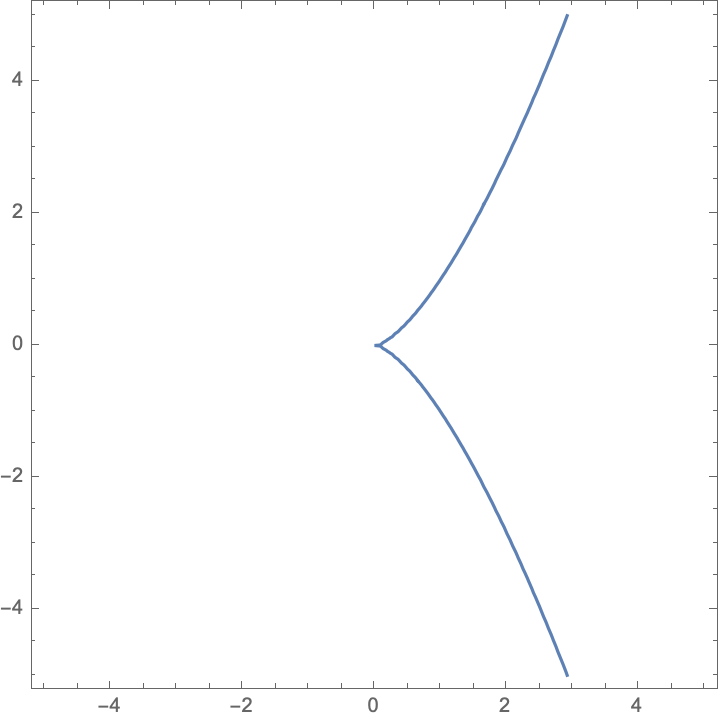
\includegraphics[width=0.5\textwidth]{Notas2/Newton's metod/nm1.png}
\end{ex}
In general, we have $f(x,y)=\sum_{(i,j)\in\Z_{\geq0}^2} a_{ij}x^iy^j$ where the $a_i$ are complex numbers, or elements in any algebraically closed field with characteristic 0.
\begin{obs}
    Although there may not be a positive convergence ratio about $(0,0)$, we can always evaluate our function in this exact point.
\end{obs}
We are looking for an expression $$y(x)=\sum_{i=0}^\infty c_{\mu_{i}}x^{\mu_i},\qquad \mu_i<\mu_j,\quad \mu_i\neq0$$
Which of course is
$$
y(x)=c_{\mu_{0}}x^{\mu_0}+\sum_{i>0}^\infty c_{\mu_{i}}x^{\mu_i}:=c_{\mu_{0}}x^{\mu_0}+\bar y$$
and we might as well take the bar and the zero off and just write $c_\mu x^\mu +y$.\par
We require that 
\begin{align*}
    0&=f(x,y)\\
    &=\sum_{(i,j)\in\Z_{\geq0}^2} a_{ij}x^iy^j\\
    &=\sum_{(ij)} a_{ij}x^i(c_\mu x^\mu +y)^j\\
    &=\sum_{(i,j)} a_{ij}x^i\sum_{k=0}^j{j\choose k} c^k_{\mu}x^{k\mu}+y^{j-k}\qquad \text{binomio de Newton}\\
    &=\sum_{(i,j)}\sum_{k=0}^j a_{ij} c^k_{\mu}x^{i+k\mu}+ y^{j-k}\\
    &=\sum_{(i,j)}a_{ij}c_\mu x^{i+j\mu}+\overline{\overline{y}}
\end{align*}
Now let $m=\min_{a_{ij}\neq0}i+j\mu$
then
$$\sum_{i+j\mu=m}a_{ij}c_\mu^jx^m=0\iff \sum_{i+j\mu=m}a_{ij}c_\mu^j=0$$
\begin{defn}
    Given a formal power series $f\in\C[[x,y]]$, the \textbf{support} of $f$ is $\supp(f)=\{(i,j):a_{ij}\neq0\}$
\end{defn}
\begin{ex}
    $$f(x,y)=x+y+x^3y^4$$
    has support
    $$\supp(f)=\{(1,0),(0,1),(3,4)\}$$
	\begin{figure}[H]
		\begin{subfigure}{.4\textwidth}
			\centering
			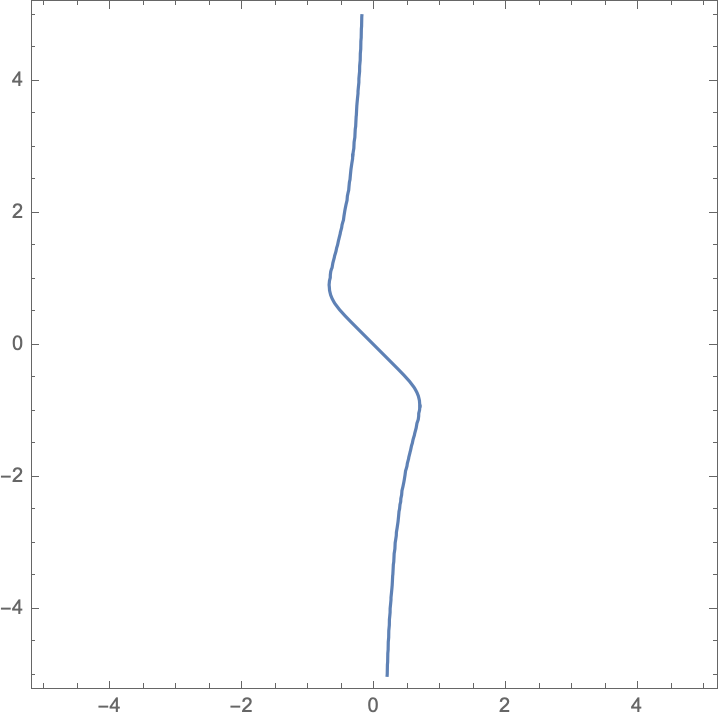
\includegraphics[width=0.9\linewidth]{Notas2/Newton's metod/nm2.png}
			\caption*{Algebraic curve}
		\end{subfigure}
		\begin{subfigure}{.4\textwidth}
			\centering
			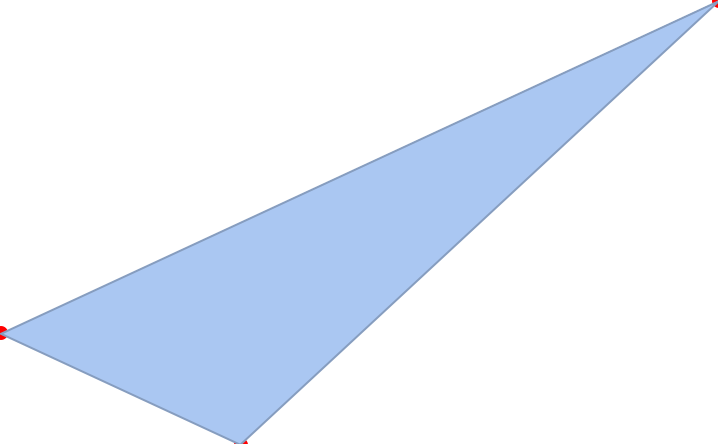
\includegraphics[width=0.9\linewidth]{Notas2/Newton's metod/nm3.png}
			\caption*{Support polygon}
		\end{subfigure}
	\end{figure}
\end{ex}

But that's actually not the Newton Polygon!
\begin{defn}
    The \textbf{Newton Polygon} of $f$ is $$\NP(f)=\conv(\supp(f)+\R_{\geq0}^2$$
\end{defn}
\begin{thm*}[Newton's lemma]
    If $f(x,y)=0$ has a solution of order $\mu$, then $(1,\mu)$ is orthogonal to a side of $\NP(f)$. (So the slope of the side of the NP is $-\frac{1}{\mu}$).\par
    Moreover, the first term is $c_\mu x^\mu$ where $c_\mu$ is a root of $f|_{L\mu}(1,c_\mu)$ where
\end{thm*}
\begin{defn}
    Let $S\subset(\Z_{\geq0})^2$.
    $$f|_S=\sum_{(i,j)\in S} a_{ij}x^iy^j$$
\end{defn}

\begin{ex}
    So for our initial example we had the polynomial $y^2-x^3$, so:
    	\begin{figure}[H]
		\begin{subfigure}{.4\textwidth}
			\centering
       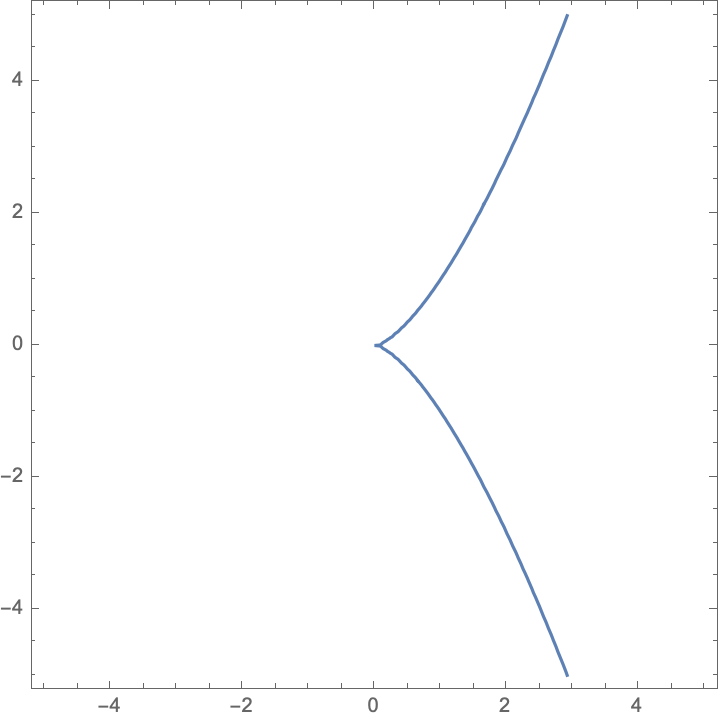
\includegraphics[width=0.9\linewidth]{Notas2/Newton's metod/nm1.png}
			\caption*{Algebraic curve}
		\end{subfigure}
		\begin{subfigure}{.4\textwidth}
			\centering
	
\includegraphics[width=0.9\linewidth]{Notas2/Newton's metod/nm4.png}
			\caption*{Newton Polygon}
		\end{subfigure}
	\end{figure}
\end{ex}
\begin{ex}[Homework] Give a parametric form for the curves
\begin{enumerate}
    \item $y^2+x+xy=0$
    \begin{proof}[Solution]
        We have $\supp(f)=\{(1,0),(1,1),(0,2)\}$ which ammounts to
        \begin{figure}[H]
		\centering\begin{subfigure}{.3\textwidth}
    \centering
	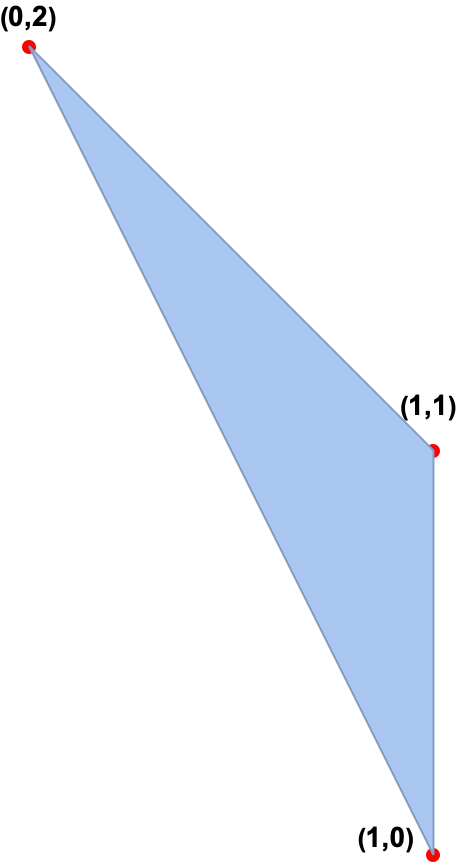
\includegraphics[width=0.7\linewidth]{Notas2/Newton's metod/H1.1.png}
			\caption*{Support polygon}
		\end{subfigure}
		\begin{subfigure}{.4\textwidth}
			\centering
			
\includegraphics[width=0.7\linewidth]{Notas2/Newton's metod/H1.2.png}
			\caption*{Newton Polygon}
		\end{subfigure}
	\end{figure}
  And we see that a side of the Newton Polygon is the line through $(0,2)$ and $(1,0)$, which has slope -2. Using our theorem, $\mu=\frac{1}{2}$ and thus the first term of our function $y(x)$ is $c_\mu$, a root of $f|_L$.\par
  Now to find $c_\mu$, we simply solve the equation $f(1,c_\mu)=0$ on the side of the Newton Polygon, which ammounts to ignoring the crossed term. So we get $0=c_\mu^2+1\iff c_\mu=\pm i$. More terms should be calculated.
    \end{proof}
    \item $y^3+xy+x^2=0$
    \begin{proof}[Solution]
    Yikes! This time we'll have
    \begin{figure}[H]
    \centering
	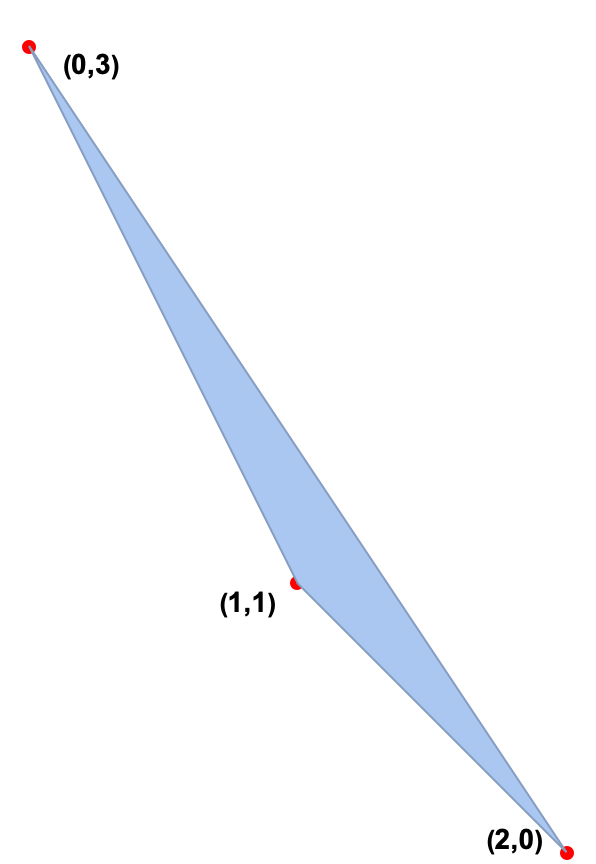
\includegraphics[width=0.3\linewidth]{Notas2/Newton's metod/H2.1.png}
    \caption*{Support polygon}
    \end{figure}
    So the Newton Polygon has two sides: which to choose?
    \end{proof}
\end{enumerate}
\end{ex}
We finally read \cite{arocailardi}, where Newton's Lemma is generalized to be applied not only to algebraic hypersurfaces like McDonald \cite{grigoriev2015tropical} did but to algebraic varieties of arbitrary codimension. It was seen how to use Newton's Lema to solve linear and nonlinear partial differential equations as in \cite{AROCA2001717} and \cite{Aroca3}.

\subsection{Excercises}
\begin{exer*}
    Consider de Pfaffian equations given by
    \begin{align}
        \omega_1&=2ydx-3xdy\\
        \omega_2&=(y^3-x^2y)dx+(x^3-2xy^2)dy
    \end{align}
    Show that there are infinite solutions of the form $y(x)=cx^{3/2}+...$, with $c\in\C\backslash\{0\}$.
\end{exer*}
\begin{proof}[Solution]
\begin{enumerate}
\item
   We wish to find $2y+3xy'$.  Suppose $y(x)=c_\mu x^\mu+\bar y$. 
    %Substituting, $$2(c_\mu x^\mu+\bar y)dx-3xd(c_\mu x^\mu+\bar y)=2(c_\mu x^\mu+\bar y)-3c_\mu x^\mu+d\bar y$$. 
    Substituting, $$0=2(c_\mu x^\mu+\bar y)-3(c_\mu x^\mu+\bar y)'=2c_\mu x^\mu+2\bar y-3c_\mu\mu x^\mu-3\bar y'=(2-3\mu)c_\mu x^\mu+2\bar y-3 \bar y'$$
    so that $\mu=3/2$.\par
    Now take $\delta y=xy'$, so that $2y-3x\delta y/x=2y-3\delta y$.\par
    For the Newton Polygon we must consider $(\underbrace{i}_x,\underbrace{j_1+j_2}_{y\text{ and }\delta y})$.
    So in the first term of our equation there is no $x$ and $j_1+j_2=1$. The same happens in the second term, so our Newton Polygon is degenerate: it is only the point $(0,1)$. We understand in this case all solutions are of the form $(x,c_\mu x^{3/2})$, for any $c_\mu$.\par
    Now consider the following plots of the vector field and its curves of solutions:
    \begin{figure}[H]
    \begin{subfigure}{0.5\textwidth}
        \centering
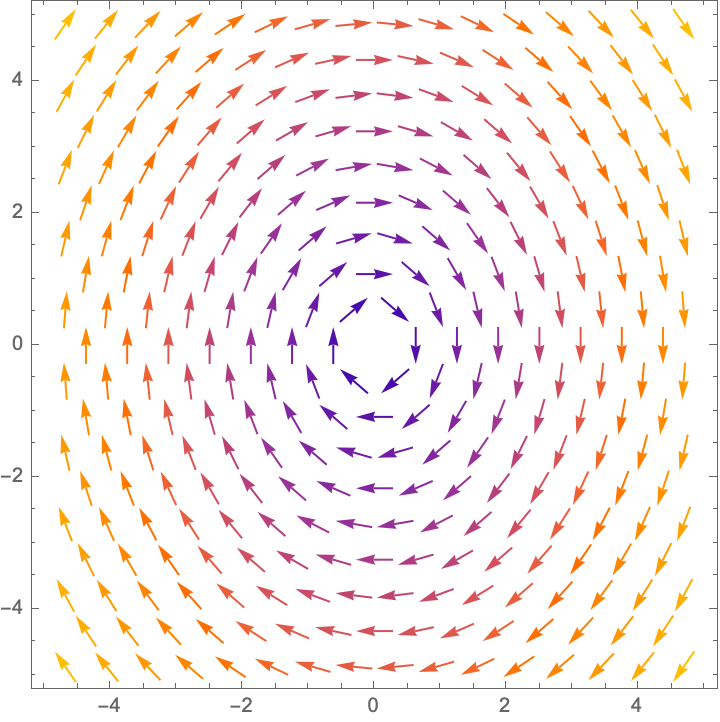
\includegraphics[width=.8\linewidth]{Notas2/vfield1.png}
        \caption{Vector field}
    \end{subfigure}
    \begin{subfigure}{0.5\textwidth}
        \centering
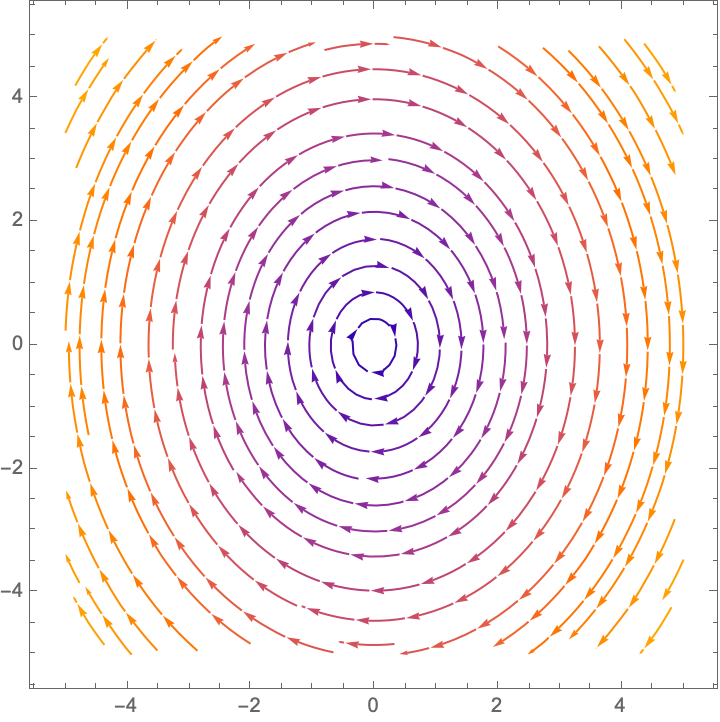
\includegraphics[width=0.8\linewidth]{Notas2/vfield2.png}
        \caption{Solution curves}
    \end{subfigure}
    \end{figure}
How can we relate this to what we have found?
\item For the second equation we only include the diagrams:
  \begin{figure}[H]
    \begin{subfigure}{0.5\textwidth}
        \centering
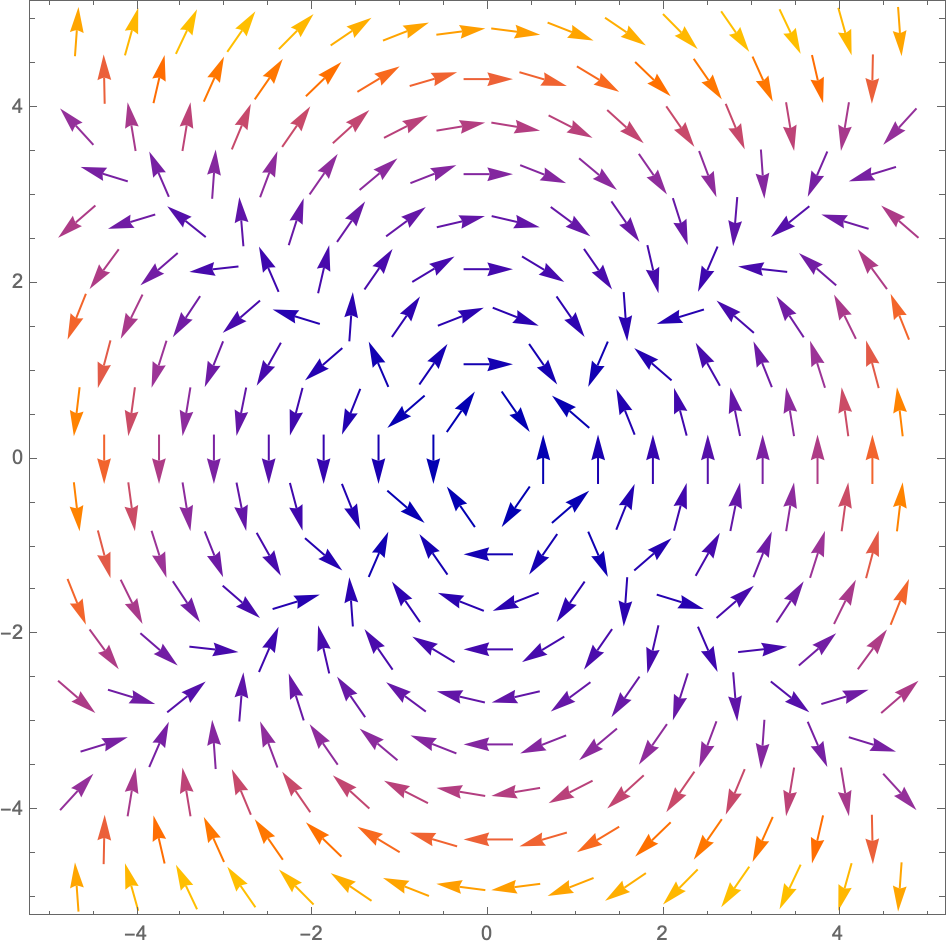
\includegraphics[width=\linewidth]{Notas2/vfield3.png}
        \caption{Vector field}
    \end{subfigure}
    \begin{subfigure}{0.5\textwidth}
        \centering
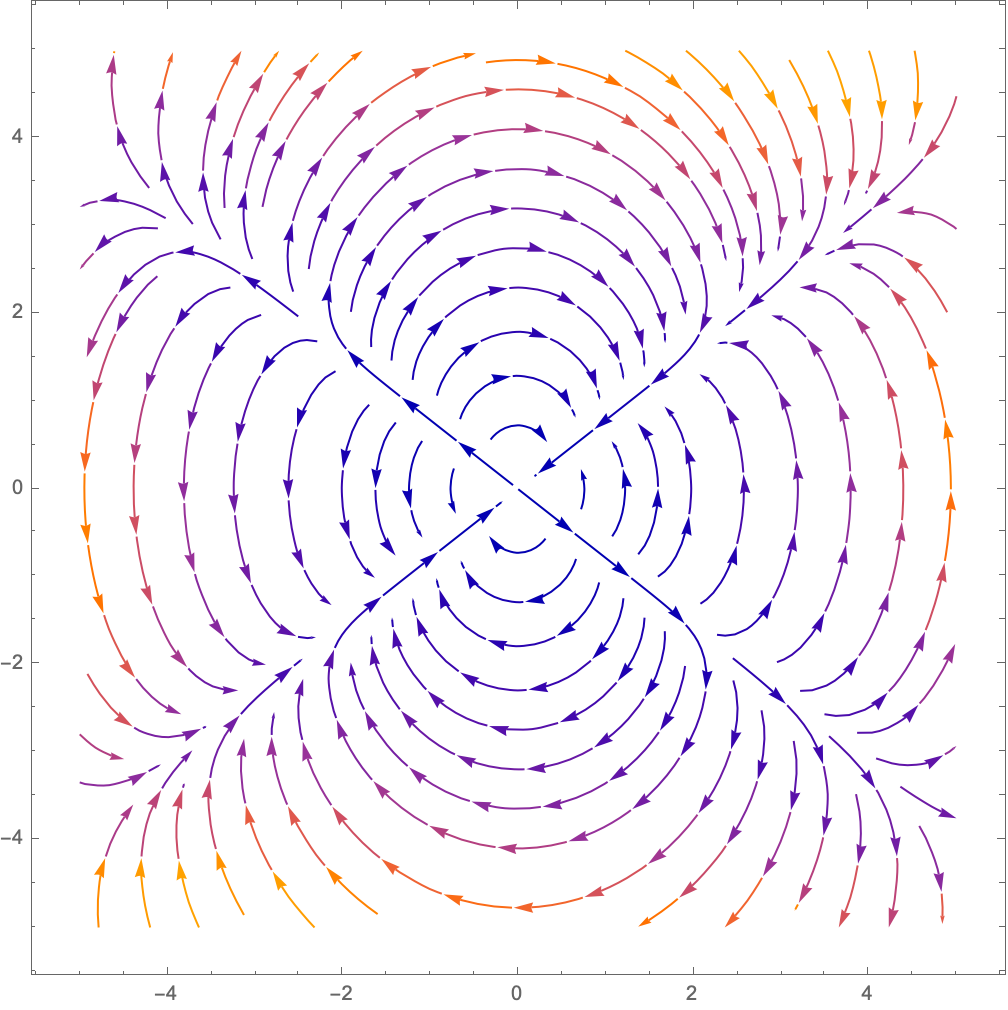
\includegraphics[width=\linewidth]{Notas2/vfield4.png}
        \caption{Solution curves}
    \end{subfigure}
    \end{figure}
\end{enumerate}
    \end{proof}
\clearpage
%\subsection{Second lecture}
%We consider curves that are orthogonal to a vector field, that is$$(a(x,y),b(x,y))\cdot\underbrace{(dx,dy)}_{\substack{\text{tangent}\\\text{to the curve}}}=0$$ According to a new computation, we obtain from a polynomial in three variables $\sum a_{ij}x^iy^j\delta y^{y_i}$ a 3-polytope for a Newton Polytope, which was projected throguh $(a,b,c)\mapsto(a,b+c)$. (...)
%And now let $\nu$ be the order function of a monomial so for example
%$$\nu(c_\mu x^\mu +y)=\mu$$
%\addcontentsline{toc}{section}{References}

\section{References}
\printbibliography[heading=none]

\end{document}